%%
%% This is file `sample-sigconf.tex',
%% generated with the docstrip utility.
%%
%% The original source files were:
%%
%% samples.dtx  (with options: `all,proceedings,bibtex,sigconf')
%% 
%% IMPORTANT NOTICE:
%% 
%% For the copyright see the source file.
%% 
%% Any modified versions of this file must be renamed
%% with new filenames distinct from sample-sigconf.tex.
%% 
%% For distribution of the original source see the terms
%% for copying and modification in the file samples.dtx.
%% 
%% This generated file may be distributed as long as the
%% original source files, as listed above, are part of the
%% same distribution. (The sources need not necessarily be
%% in the same archive or directory.)
%%
%%
%% Commands for TeXCount
%TC:macro \cite [option:text,text]
%TC:macro \citep [option:text,text]
%TC:macro \citet [option:text,text]
%TC:envir table 0 1
%TC:envir table* 0 1
%TC:envir tabular [ignore] word
%TC:envir displaymath 0 word
%TC:envir math 0 word
%TC:envir comment 0 0
%%
%% The first command in your LaTeX source must be the \documentclass
%% command.
%%
%% For submission and review of your manuscript please change the
%% command to \documentclass[manuscript, screen, review]{acmart}.
%%
%% When submitting camera ready or to TAPS, please change the command
%% to \documentclass[sigconf]{acmart} or whichever template is required
%% for your publication.
%%
%%
% \documentclass[sigconf]{acmart}
\let\Bbbk\relax
\documentclass[sigconf]{acmart}
\usepackage{amsmath}
\let\Bbbk\relax  
\usepackage{amssymb}
\usepackage{enumitem}
%%
%% \BibTeX command to typeset BibTeX logo in the docs
\AtBeginDocument{%
  \providecommand\BibTeX{{%
    Bib\TeX}}}

%% Rights management information.  This information is sent to you
%% when you complete the rights form.  These commands have SAMPLE
%% values in them; it is your responsibility as an author to replace
%% the commands and values with those provided to you when you
%% complete the rights form.
\setcopyright{acmlicensed}
% \copyrightyear{2018}
% \acmYear{2018}
% \acmDOI{XXXXXXX.XXXXXXX}
% %% These commands are for a PROCEEDINGS abstract or paper.
% \acmConference[Conference acronym 'XX]{Make sure to enter the correct
%   conference title from your rights confirmation email}{June 03--05,
%   2018}{Woodstock, NY}
% %%
% %%  Uncomment \acmBooktitle if the title of the proceedings is different
% %%  from ``Proceedings of ...''!
% %%
% %%\acmBooktitle{Woodstock '18: ACM Symposium on Neural Gaze Detection,
% %%  June 03--05, 2018, Woodstock, NY}
% \acmISBN{978-1-4503-XXXX-X/2018/06}

% \copyrightyear{2026}
% \acmYear{2026}
% \setcopyright{cc}
% \setcctype{by}
% \acmConference[WWW '26] {Proceedings of the ACM Web Conference 2026}{April 13--17, 2026}{Dubai, United Arab Emirates.}
% \acmBooktitle{Proceedings of the ACM Web Conference 2026 (WWW '26), April 13--17, 2026, Dubai, United Arab Emirates}
% \acmISBN{979-8-4007-2307-0/2026/04}
% \acmDOI{10.1145/3774904.3792191}

% 1 Authors, replace the red X's with your assigned DOI string during the rightsreview eform process.
% 2 Your DOI link will become active when the proceedings appears in the DL.
% 3 Retain the DOI string between the curly braces for uploading your presentation video.

\settopmatter{printacmref=true}
% \settopmatter{authorsperrow=4}

%%
%% Submission ID.
%% Use this when submitting an article to a sponsored event. You'll
%% receive a unique submission ID from the organizers
%% of the event, and this ID should be used as the parameter to this command.
%%\acmSubmissionID{123-A56-BU3}

%%
%% For managing citations, it is recommended to use bibliography
%% files in BibTeX format.
%%
%% You can then either use BibTeX with the ACM-Reference-Format style,
%% or BibLaTeX with the acmnumeric or acmauthoryear sytles, that include
%% support for advanced citation of software artefact from the
%% biblatex-software package, also separately available on CTAN.
%%
%% Look at the sample-*-biblatex.tex files for templates showcasing
%% the biblatex styles.
%%

%%
%% The majority of ACM publications use numbered citations and
%% references.  The command \citestyle{authoryear} switches to the
%% "author year" style.
%%
%% If you are preparing content for an event
%% sponsored by ACM SIGGRAPH, you must use the "author year" style of
%% citations and references.
%% Uncommenting
%% the next command will enable that style.
%%\citestyle{acmauthoryear}


%%
%% end of the preamble, start of the body of the document source.
\begin{document}

%%
%% The "title" command has an optional parameter,
%% allowing the author to define a "short title" to be used in page headers.
\title{Plan Then Retrieve: Reinforcement Learning-Guided Complex Reasoning over Knowledge Graphs}

%%
%% The "author" command and its associated commands are used to define
%% the authors and their affiliations.
%% Of note is the shared affiliation of the first two authors, and the
%% "authornote" and "authornotemark" commands
%% used to denote shared contribution to the research.
\author{Yanlin Song}
\authornote{Equal contribution.}
% \authornote{This work is conducted during an internship at Alibaba Group.}
\affiliation{%
  \department{School of Computer Science}
  \institution{Wuhan University}
  \city{Wuhan}
  \country{China}
}
\email{songyanlin@whu.edu.cn}

\author{Ben Liu}
\authornotemark[1]
\affiliation{%
  \institution{Ant Group}
  \city{Hangzhou}
  \country{China}
}
\email{keli.lb@antgroup.com}


\author{Víctor Gutiérrez-Basulto}
\affiliation{%
  \department{School of Computer Science and Informatics}
  \institution{Cardiff University}
  \city{Cardiff}
  \country{UK}
}
\email{GutierrezBasultoV@cardiff.ac.uk}


\author{Zhiwei Hu}
\affiliation{%
  \department{College of Information Science and Engineering}
  \institution{Shanxi Agricultural University}
  \city{Taiyuan}
  \country{China}
}
\email{zhiweihu@whu.edu.cn}

\author{Qianqian Xie}
\authornotemark[2]
\affiliation{%
  \department{School of Artificial Intelligence}
  \institution{Wuhan University}
  \city{Wuhan}
  \country{China}
}
\affiliation{%
  \department{Center for Language and Information Research}
  \institution{Wuhan University}
  \city{Wuhan}
  \country{China}
}
\email{xieq@whu.edu.cn}

\author{Min Peng}
\authornote{Corresponding Author.}
\affiliation{%
  \department{School of Artificial Intelligence}
  \institution{Wuhan University}
  \city{Wuhan}
  \country{China}
}
\affiliation{%
  \department{Center for Language and Information Research}
  \institution{Wuhan University}
  \city{Wuhan}
  \country{China}
}
\email{pengm@whu.edu.cn}


\author{Sophia Ananiadou}
\affiliation{%
  \department{School of Computer Science}
  \institution{University of Manchester}
  \city{Manchester}
  \country{UK}
}
\email{sophia.ananiadou@manchester.ac.uk}

\author{Jeff Z. Pan}
\affiliation{%
  \department{ILCC, School of Informatics}
  \institution{University of Edinburgh}
  \city{Edinburgh}
  \country{UK}
}
\email{j.z.pan@ed.ac.uk}

\newcommand{\todo}[1]{\textcolor{red}{[todo: #1]}}

\newcommand{\vic}[1]{\textcolor{black}{#1}}
\newcommand{\zhiwei}[1]{\textcolor{black}{#1}}
%
\newcommand{\nb}[1]{\textcolor{red}{$\blacktriangleright$}\footnote{\textcolor{blue}{#1}}}

\newcommand{\paperComment}[3]{{\color{#2}\par\noindent\fbox{\parbox{0.97\linewidth}{{\sf #1:} #3}}\newline}}
 \newcommand{\victor}[1]{\paperComment{Victor}{purple!50!black}{#1}}
%%

%%
%% By default, the full list of authors will be used in the page
%% headers. Often, this list is too long, and will overlap
%% other information printed in the page headers. This command allows
%% the author to define a more concise list
%% of authors' names for this purpose.
\renewcommand{\shortauthors}{Yanlin Song et al.}

%%
%% The abstract is a short summary of the work to be presented in the
%% article.
\begin{abstract}
% Although Large Language Models (LLMs) possess strong reasoning capabilities, they are prone to hallucinations constrained by a lack of precise knowledge~\cite{yao2023llm}. To address this issue, Knowledge Graphs (KGs), storing a vast amount of knowledge in the form  symbolic triples have been integrated with LLMs. This integration has played a key role in the development of state-of-the art approaches to \emph{knowledge graph question answering (KGQA)}. However, these methods still struggle to fully leverage the knowledge in KGs and the reasoning capabilities of LLMs in more complex instances. This is due two main reasons. First, they lack the ability to adaptively judge whether the knowledge in KGs is sufficient, as it is difficult for KGs in reality to contain all the triples required for answering questions. 
% Second, 
% % they overlook the importance of interaction between global planning and tool scheduling, leading to retrieval failures even when the answers are available in KGs. 
% the reasoning process for dealing with complex scenarios is largely constrained to local decision-making and overlook the importance of multi-step planning, leading to retrieval failures even when the answers are available in KGs. 
% In this paper, we propose Graph-RFT, a multi-reward two-stage reinforcement learning framework that adopts a new “plan-KGsearch-and-Websearch-during-think” paradigm. Inspired by Cartesian principles\cite{descartes1901discourse}, we plan the execution steps with logic functions, which helps the model to understand the interaction between problem decomposition and tool invocation. Graph-RFT employs a systematic training framework, beginning with distilling high quality CoT trajectories for supervised fine-tuning (SFT) to enhance the LLMs’ capability on multi-step planning. 
% % reasonable decomposition. 
% Furthermore, we use reinforcement learning incorporating multi-rewards to improve the models’ capabilities for   learning how and when to retrieve structured KG as well as unstructured web documents. Experiments on single-hop and multi-hop benchmarks demonstrate that Graph-RFT significantly outperforms existing approaches, particularly in complex, multi-hop reasoning scenarios.
Knowledge Graph Question Answering (KGQA) aims to answer natural language questions by reasoning over structured knowledge graphs (KGs). While large language models (LLMs) have advanced KGQA through their strong reasoning capabilities, existing methods continue to struggle to fully exploit both the rich knowledge encoded in KGs and the reasoning capabilities of LLMs, particularly in complex scenarios. 
They often assume complete KG coverage and lack mechanisms to judge when external information is needed, and their reasoning remains locally myopic, failing to maintain coherent multi-step planning, leading to reasoning failures even when relevant knowledge exists.
We propose \textbf{Graph-RFT}, a novel two-stage reinforcement fine-tuning KGQA framework with a “plan–KGsearch–and–Websearch–during–think” paradigm, that enables LLMs to perform autonomous planning and adaptive retrieval scheduling across KG and web sources under incomplete knowledge conditions. 
Graph-RFT introduces a chain-of-thought (CoT) fine-tuning method with a customized plan–retrieval dataset activates structured reasoning and resolves the GRPO cold-start problem.
It then introduces a novel plan–retrieval guided reinforcement learning process integrates explicit planning and retrieval actions with a multi-reward design, enabling coverage-aware retrieval scheduling.
It employs a Cartesian-inspired planning module to decompose complex questions into ordered sub-questions, and logical expression to guide tool invocation for globally consistent multi-step reasoning.
This reasoning–retrieval process is optimized with a multi-reward combining outcome and retrieval-specific signals, enabling the model to learn when and how to combine KG and web retrieval effectively.
Experiments on multiple KGQA benchmarks demonstrate that Graph-RFT achieves superior performance over strong baselines, even with smaller LLM backbones, and substantially improves complex question decomposition, factual coverage, and tool coordination. 

%\vic{Although large language models (LLMs) exhibit strong reasoning abilities, they are still prone to hallucinations due to their lack of precise factual knowledge~\cite{yao2023llm}. To mitigate this limitation, knowledge graphs (KGs), which store structured knowledge in the form of symbolic triples, have been integrated with LLMs. This integration has driven recent advances in \emph{knowledge graph question answering (KGQA)}. However, existing methods continue to struggle to fully exploit both the rich knowledge encoded in KGs and the reasoning capabilities of LLMs, particularly in complex scenarios.These challenges stem from two main issues. First, current systems lack the ability to adaptively determine whether the knowledge contained in a KG is sufficient to answer a given question, as real-world KGs are inevitably incomplete. Second, their reasoning processes are often confined to local decision-making, overlooking the importance of multi-step planning. As a result, they frequently fail to retrieve correct answers even when the necessary information exists within the KG.To address these limitations, we propose \textbf{Graph-RFT}, a multi-reward, two-stage reinforcement learning framework that adopts a novel “plan–KGsearch–and–Websearch–during–think” paradigm. Inspired by Cartesian principles~\cite{descartes1901discourse}, Graph-RFT employs logical functions to plan execution steps, enabling the model to better capture the interplay between problem decomposition and tool invocation. The framework begins with distillation of high-quality chain-of-thought  trajectories for supervised fine-tuning, enhancing the LLM’s ability to perform coherent multi-step reasoning. Subsequently, reinforcement learning with multi-reward signals is applied to improve the model’s capacity to decide when and how to retrieve both structured KG knowledge and unstructured web information. Experimental results on single-hop and multi-hop benchmarks demonstrate that Graph-RFT substantially outperforms existing methods, particularly in complex, multi-hop reasoning scenarios.}

% \vspace{0.2cm} \noindent 
% \textbf{Relevance for WWW.} Graph-RFT is a key task for the integration of LLMs, KGs and web application, which is a scientific challenge within the scope of the Semantics and Knowledge Track.

\end{abstract}


% \textbf{Relevance for WWW.} Graph-RFT is a key task for the integration of LLMs, KGs and web application, which is a scientific challenge within the scope of the Semantics and Knowledge Track.
%%
%% The code below is generated by the tool at http://dl.acm.org/ccs.cfm.
%% Please copy and paste the code instead of the example below.
% %%
% \begin{CCSXML}
% <ccs2012>
%  <concept>
%   <concept_id>00000000.0000000.0000000</concept_id>
%   <concept_desc>Do Not Use This Code, Generate the Correct Terms for Your Paper</concept_desc>
%   <concept_significance>500</concept_significance>
%  </concept>
%  <concept>
%   <concept_id>00000000.00000000.00000000</concept_id>
%   <concept_desc>Do Not Use This Code, Generate the Correct Terms for Your Paper</concept_desc>
%   <concept_significance>300</concept_significance>
%  </concept>
%  <concept>
%   <concept_id>00000000.00000000.00000000</concept_id>
%   <concept_desc>Do Not Use This Code, Generate the Correct Terms for Your Paper</concept_desc>
%   <concept_significance>100</concept_significance>
%  </concept>
%  <concept>
%   <concept_id>00000000.00000000.00000000</concept_id>
%   <concept_desc>Do Not Use This Code, Generate the Correct Terms for Your Paper</concept_desc>
%   <concept_significance>100</concept_significance>
%  </concept>
% </ccs2012>
% \end{CCSXML}

% \ccsdesc[500]{Do Not Use This Code~Generate the Correct Terms for Your Paper}
% \ccsdesc[300]{Do Not Use This Code~Generate the Correct Terms for Your Paper}
% \ccsdesc{Do Not Use This Code~Generate the Correct Terms for Your Paper}
% \ccsdesc[100]{Do Not Use This Code~Generate the Correct Terms for Your Paper}
\begin{CCSXML}
<ccs2012>
   <concept>
       <concept_id>10010147.10010178.10010187.10010188</concept_id>
       <concept_desc>Computing methodologies~Semantic networks</concept_desc>
       <concept_significance>300</concept_significance>
       </concept>
 </ccs2012>
\end{CCSXML}

\ccsdesc[300]{Computing methodologies~Semantic networks}


%%
%% Keywords. The author(s) should pick words that accurately describe
%% the work being presented. Separate the keywords with commas.
\keywords{Knowledge Graph Question Answering, Large Language Model, Reinforcement Learning}
%% A "teaser" image appears between the author and affiliation
%% information and the body of the document, and typically spans the
%% page.

% \received{20 February 2007}
% \received[revised]{12 March 2009}
% \received[accepted]{5 June 2009}

%%
%% This command processes the author and affiliation and title
%% information and builds the first part of the formatted document.
\maketitle

\section{Introduction}
% Large language models (LLMs) have demonstrated remarkable capabilities in natural language understanding, reasoning and generation \cite{hendrycks2020measuring, clark2018think, guo2025deepseek}, %However, they still
% but they suffer from hallucinations due to %the lack of 
% insufficient and imprecise parametric knowledge \cite{yao2023llm, huang2025survey, li2023halueval}. 
% Knowledge Graphs (KGs) encompass a massive amout of triples, providing explicit and explainable knowledge which is utilized by many researchers as knowledge sources for LLMs when dealing with various tasks, such as Knowledge Graph Question Answering (KGQA) 
% \cite{sun2023think, jiang2023structgpt, tan2025paths, ma2025debate, liu2025symagent}. 
% The integration of KG and LLM enables the development of numerous web-based applications, including search engine recommendation~\cite{khorashadizadeh2024research, zhao2024breaking}, and social networks~\cite{zeng2024large}.

%\vic{Large language models (LLMs) have demonstrated remarkable capabilities in natural language understanding, reasoning, and generation~\cite{hendrycks2020measuring, clark2018think, guo2025deepseek, shi2025search}. However, they remain susceptible to hallucinations caused by insufficient and imprecise parametric knowledge~\cite{yao2023llm, huang2025survey, li2023halueval}.To overcome this limitation, knowledge graphs (KGs), which store vast amounts of explicit, structured, and explainable knowledge in the form of triples, have been employed as external knowledge sources to enhance LLM performance on tasks requiring precise factual information~\cite{sun2023think, jiang2023structgpt, tan2025paths, ma2025debate, liu2025symagent, xue2024decompose}.This integration has also catalyzed the development of a wide range of web-based applications, including intelligent search and recommendation systems~\cite{khorashadizadeh2024research, zhao2024breaking} as well as  social networks~\cite{zeng2024large}.}

Knowledge Graph Question Answering (KGQA) aims to answer natural language questions by reasoning over structured knowledge graphs (KGs) that store explicit, factual knowledge in the form of triples. KGQA plays a central role in web-based intelligent systems such as search, recommendation, and social platforms~\cite{khorashadizadeh2024research, zhao2024breaking, zeng2024large, xie2023pixiu, xie2024finben, xie2025medical, wang2023pre}, where accurate and explainable reasoning over structured data is crucial.
Recent advances in large language models (LLMs) have transformed natural language understanding, reasoning, and generation~\cite{hendrycks2020measuring, clark2018think, guo2025deepseek, shi2025search, liu2025visual}. Leveraging their strong generalization and reasoning capabilities, recent KGQA methods increasingly rely on LLMs, integrating knowledge graphs as structured, verifiable knowledge sources to enhance factual precision and interpretability~\cite{sun2023think, jiang2023structgpt, tan2025paths, ma2025debate, liu2025symagent, xue2024decompose}.

Existing LLM-based KGQA approaches fall into two paradigms: \textbf{semantic parsing (SP)}, which translates natural questions into executable logical queries (e.g., SPARQL) and runs them over a KG \cite{li2023few, luo2023chatkbqa, xu2024generate}, and \textbf{retrieval-augmented generation (RAG)}, which retrieves relevant KG triples to condition an LLM’s generation \cite{tan2025paths, xu2024generate}.
Despite substantial progress, both paradigms struggle in complex settings for two main reasons.
First, they lack a reliable mechanism to judge whether a KG contains the facts necessary to answer a question. SP and RAG methods commonly assume that all required triples are present in the KG, a strong and unrealistic assumption for manually curated graphs. When coverage is incomplete, SP fails to produce correct executable queries, and RAG offers no built-in way to refine retrieval or to decide when to consult external (unstructured) sources.
Second, these methods often lack the ability to perform coherent multi-step planning and adaptive retrieval scheduling. For example in Figure \ref{fig:intro}(2), an LLM may correctly decompose a question into ``Which screenwriters wrote Analyze That?'' and retrieve ``Harold Ramis,'' but then fail to continue the planned decomposition and instead reformulates the follow-up as ``When was Harold Ramis released?'', confusing the person with a film title. This failure stems from constrained local decision-making and an absence of coherent multi-step planning, which leads to retrieval and reasoning errors even when the KG contains the necessary facts. 
The comparison for previous work and Graph-RFT is in Table \ref{intro:compare}.


\begin{figure}[t]
    \centering
    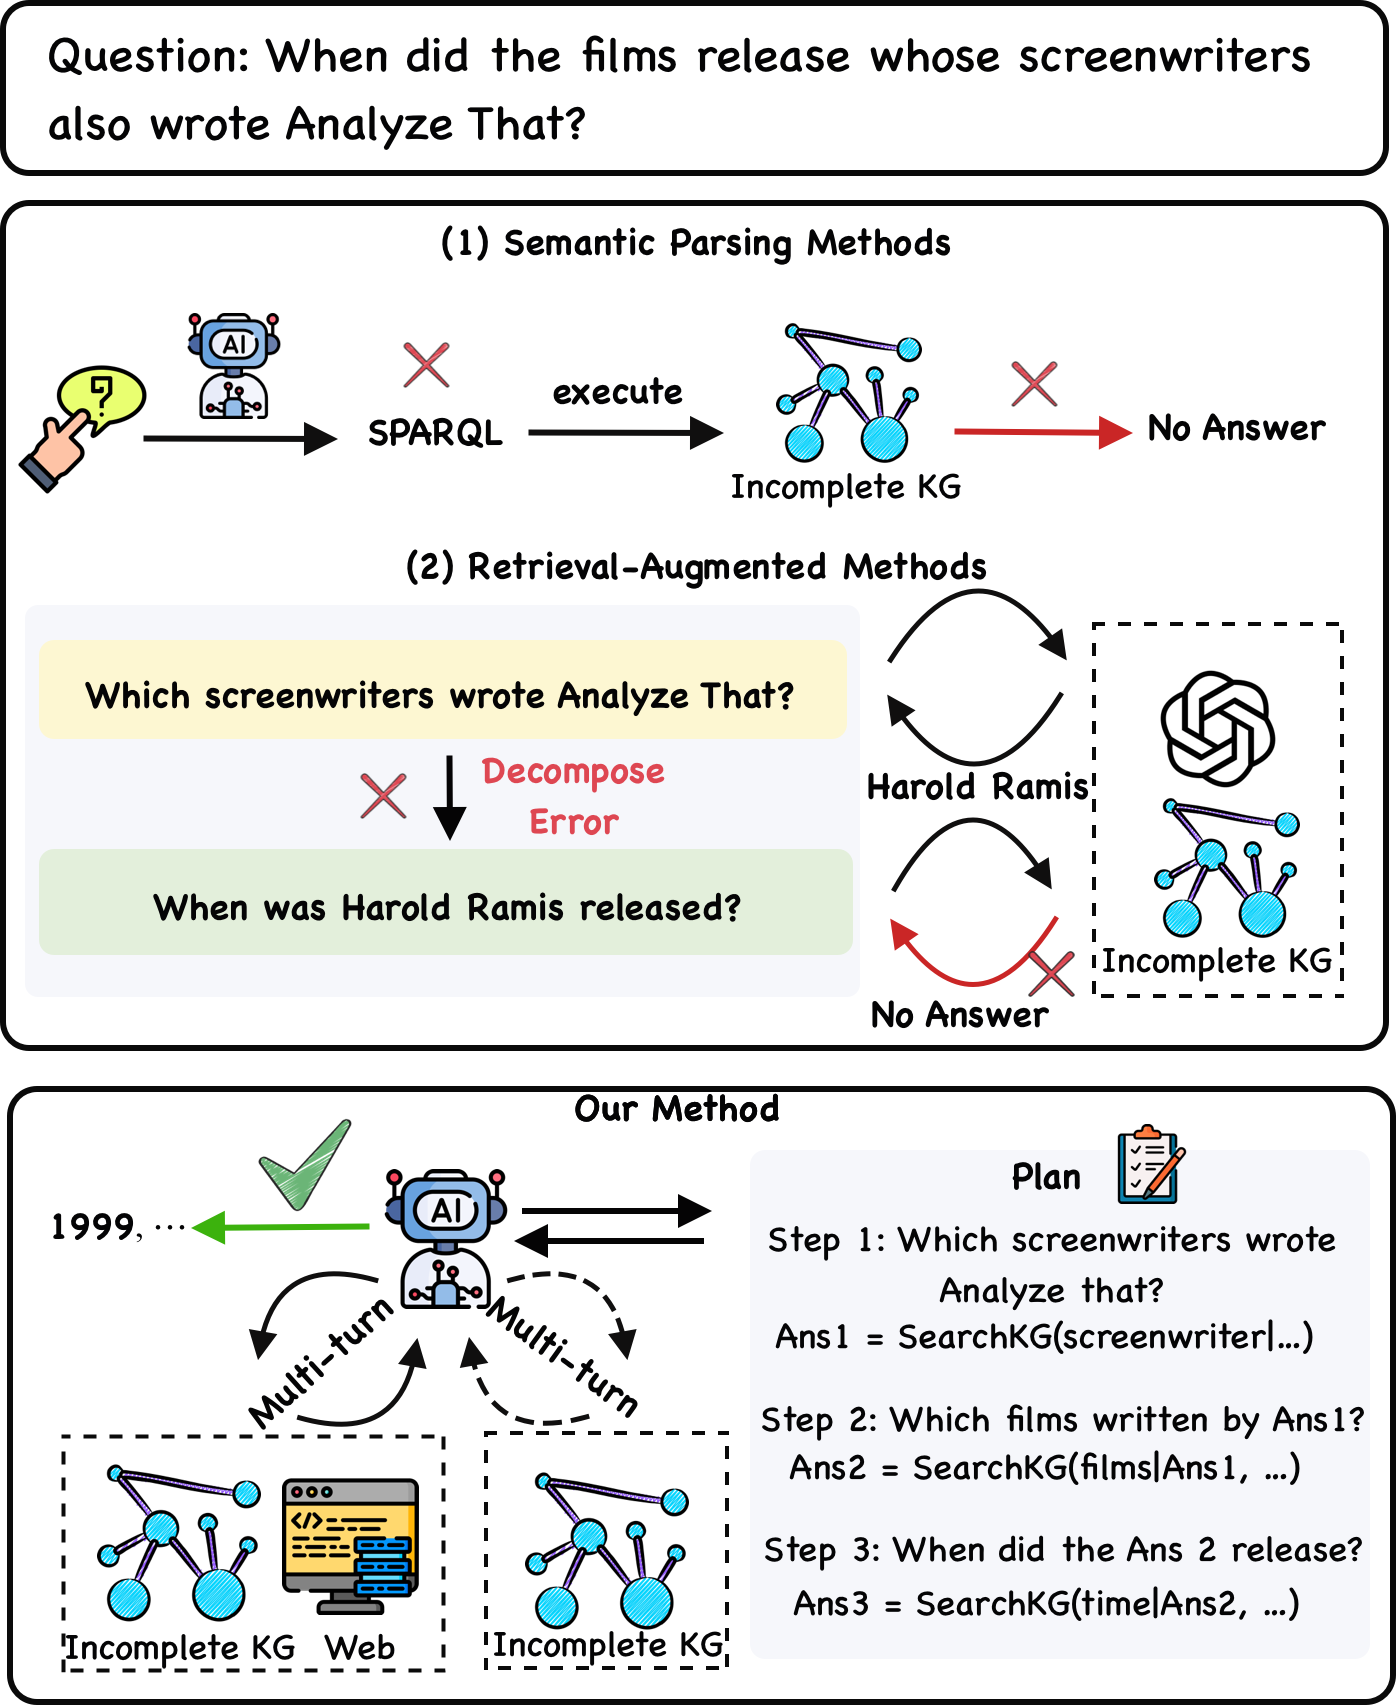
\includegraphics[width=0.95\linewidth]{intro.png}
    \caption{The comparison of Semantic Parsing, Retrieval-Augmented Methods, and Graph-RFT. }
    \label{fig:intro}
\end{figure}

\begin{sloppypar}
% To address these challenges, we propose Graph-RFT, a novel two-stage reinforcement fine-tuning framework to promote model’s capabilities in autonomous planning and adaptive scheduling of retrieval across different tools (KG search tool and web search tool) in the incomplete KGs.
% % a dynamic knowledge graph-enhanced multi-reward reinforcement learning framework that boosts the model’s capabilities in autonomous planning and adaptive scheduling of retrieval across different tools in the incomplete KG.
% First, in Section 4.1, we use a customized high-quality plan-retrieval dataset to activate the model’s planning and reasoning abilities while resolving the GRPO cold-start issue. Second, we integrate explicit planning steps and retrieval content into the reasoning loop via the <plan><relation\_search><neighbor\_search><web\_search> template. For the design of the plan module, we adopt a Cartesian-inspired approach to decompose complex questions into sub-questions ordered by logical dependencies, and design logical expressions to guide the KG retrieval tools invocation and represent relationships between sub-questions 
% % (an atomic, meaningfully indivisible small question derived from breaking down a complex question)
% % begins by carefully analyzing the question and breaking it down into a set of atomic sub-questions that follow a logical dependency structure. The system then answers these sub-questions step by step, starting with the most basic ones that do not rely on any prior information. As each sub-question is resolved, its answer becomes part of the context used to guide the retrieval and resolution of the next, more dependent sub-question. The final answer is synthesized only after all necessary sub-questions have been addressed.
% , strengthening the model’s grasp of both complex question decomposition and the overall retrieval process in global planning. For each execution step derived from the plan, we invoke the relation search tool and neighbor search tool for KG retrieval; when KG knowledge is insufficient to answer a sub-question, we further call the web search tool to query external documents, with the query results supplementing the KG. Under the  template mentioned above, we apply GRPO to train the model, further enhancing its planning, reasoning, and retrieval potential. Furthermore, we incorporate retrieval-specific rewards alongside outcome rewards, which guides the model on whether to use web document retrieval alongside KG retrieval, improves the KG and web document retrieval processes themselves and enables the model to fully learn how and when to retrieve structured KG knowledge and unstructured external document knowledge in incomplete scenario.

To address these challenges, we propose Graph-RFT, a novel two-stage reinforcement fine-tuning framework designed to enhance an LLM’s capabilities in autonomous planning and adaptive retrieval scheduling across multiple tools (specifically, KG search and web search) under conditions of incomplete KGs.
In the first stage (Section~\ref{data_collection}), we introduce a chain-of-thought (CoT)~\cite{wei2022chain} fine-tuning method that uses a customized plan–retrieval dataset to explicitly train the model to decompose questions, formulate plans, and select retrieval tools. This stage not only activates the model’s reasoning and planning capabilities but also resolves the GRPO \cite{guo2025deepseek} cold-start problem, enabling stable and meaningful reinforcement rollouts. 

In the second stage (Section~\ref{second_stage}), we propose a plan–retrieval guided reinforcement learning method that integrates explicit planning steps and retrieval actions into the model’s reasoning loop, and learns a coverage-aware retrieval policy that dynamically coordinates knowledge graph and web search under incomplete KG conditions.
It uses a structured template
$\langle$\textit{plan}$\rangle\langle$\textit{relation\_search}$\rangle\langle$\textit{neighbor\_search}$\rangle$$\langle$\textit{web\_search}$\rangle$, to explicitly let the model to alternate between symbolic planning and retrieval actions. 
The planning module draws inspiration from Cartesian principles~\cite{descartes1901discourse}, breaking complex questions into logically ordered sub-questions. We further employ logical expressions to represent dependencies among sub-questions and guide the invocation of KG retrieval tools, ensuring globally coherent multi-step reasoning and controllable retrieval flow. For each planned execution step, Graph-RFT invokes both relation-search and neighbor-search tools to perform KG retrieval; when the KG lacks sufficient coverage, the model automatically triggers web search to acquire supplementary unstructured evidence.
To optimize the reasoning–retrieval process, we apply a GRPO-based reinforcement learning with a novel multi-reward design: an outcome reward measuring factual correctness and a retrieval-specific reward that evaluates retrieval coverage, precision, and timing.
This formulation encourages the model to learn when and how to combine KG and web retrieval, overcoming the limitations of prior SP and RAG methods that assume complete KGs and the absence of coherent multi-step planning.
%we integrate explicit planning steps and retrieval actions into the reasoning loop \ref{rollout} through a structured template:$\langle$\textit{plan}$\rangle\langle$\textit{relation\_search}$\rangle\langle$\textit{neighbor\_search}$\rangle$$\langle$\textit{web\_search}$\rangle$.For the design of the planning module, we draw inspiration from Cartesian principles to decompose complex questions into logically ordered sub-questions. Logical expressions \ref{functions} are then employed to guide the invocation of KG retrieval tools and to represent the dependencies among sub-questions. This approach strengthens the model’s ability to perform coherent multi-step planning and manage the global retrieval process.For each execution step derived from the plan, Graph-RFT invokes both the relation-search and neighbor-search tools to perform KG retrieval. When the available KG knowledge is insufficient to answer a sub-question, the model automatically calls the web-search tool to retrieve relevant external documents, which serve as supplementary knowledge.Under the proposed template, we apply GRPO-based reinforcement learning to further enhance the model’s planning, reasoning, and retrieval capabilities. Additionally, we introduce retrieval-specific rewards \ref{rewards} alongside traditional outcome rewards, enabling the model to learn not only whether to use web retrieval in combination with KG retrieval, but also how to optimize each process. This dual-reward design helps the model master when and how to retrieve both structured KG knowledge and unstructured external information in settings with incomplete knowledge coverage.

% \begin{table}[htbp]
%   \centering
%   \caption{Comparison for main characteristics of previous SP, RAG methods with our Graph-RFT.}
%   \label{intro:compare}
%   \resizebox{\linewidth}{!}{
%     \begin{tabular}{c|cc|cccc}
%       \toprule
%       \textbf{Class} &\textbf{Algorithm} & \textbf{Paradigm} & \textbf{Incomplete KG} &\textbf{Global Planning} & \textbf{Decompose Problems} & \textbf{KG Interaction} \\
%       \midrule
%       SP &RGR-KBQA \cite{feng2025rgr} & SFT & \times & \times & \times & \times \\
%       SP &Rule-KBQA \cite{zhang2025rule} & SFT & \times & \times & \times & \times \\\midrule
%       RAG &PoG \cite{tan2025paths}& ICL & \times & \times & \checkmark & \checkmark\\
%       RAG &DoG \cite{ma2025debate} & ICL & \times & \times & \checkmark & \checkmark \\
%       RAG &KG-Agent \cite{jiang2024kg} & SFT & \times & \times & \checkmark & \checkmark \\\midrule
%       Our Method &Graph-RFT& SFT \& RL & \checkmark & \checkmark & \checkmark & \checkmark\\
%       \bottomrule
%     \end{tabular}
%   }
% \end{table}

\begin{table}[htbp]
  \centering
  \caption{Comparison for main characteristics of previous SP, RAG methods with our Graph-RFT.}
  \label{intro:compare}
  \resizebox{\linewidth}{!}{
    \begin{tabular}{c|cc|cccc}
      \toprule
      \textbf{Class} & \textbf{Algorithm} & \textbf{Paradigm} & \textbf{Incomplete KG} & \textbf{Global Planning} & \textbf{Decompose Problems} & \textbf{KG Interaction} \\
      \midrule
      SP & RGR-KBQA \cite{feng2025rgr} & SFT & $\times$ & $\times$ & $\times$ & $\times$ \\
      SP & Rule-KBQA \cite{zhang2025rule} & SFT & $\times$ & $\times$ & $\times$ & $\times$ \\
      \midrule
      RAG & PoG \cite{tan2025paths} & ICL & $\times$ & $\times$ & $\checkmark$ & $\checkmark$ \\
      RAG & DoG \cite{ma2025debate} & ICL & $\times$ & $\times$ & $\checkmark$ & $\checkmark$ \\
      RAG & KG-Agent \cite{jiang2024kg} & SFT & $\times$ & $\times$ & $\checkmark$ & $\checkmark$ \\
      \midrule
      Our Method & Graph-RFT & SFT \& RL & $\checkmark$ & $\checkmark$ & $\checkmark$ & $\checkmark$ \\
      \bottomrule
    \end{tabular}
  }
\end{table}


Our main contributions are as follows:
\end{sloppypar}
% \begin{itemize}
% \item We propose Graph-RFT, a novel two-stage reinforcement fine-tuning framework for complex reasoning over incomplete knowledge graphs, effectively integrating the strengths of  both LLMs and external knowledge, including KGs and web documents. By automatically calling pre-defined action tools, Graph-RFT converts natural language questions into multi-step interactive processes that involve logical functions, enabling the mutual enhancement of KGs and LLMs. 
% \item We develop a multi-reward reinforcement learning approach that integrates both graph, web retrieval and penalty rewards into the conventional outcome-based reward framework. By incorporating feedback, the approach guides Graph-RFT for determining how and when to retrieve from knowledge graph and web documents.
% \item Experimental results on several widely used complex reasoning datasets demonstrate that Graph-RFT with weak LLM backbones (i.e., 7B series) achieves better or comparable performance compared to strong baselines. Comprehensive empirical analyses validate the effectiveness of Graph-RFT in multiple aspects, including complex question decomposition planning, missing factual triples identification and different tools invocation.
% \end{itemize}
%\vic{
\begin{itemize}[itemsep=0.5ex, leftmargin=3mm]
\item  We introduce Graph-RFT, a novel two-stage reinforcement fine-tuning framework for complex reasoning over incomplete KGs. It introduces the novel CoT-based fine-tuning method to activate planning and reasoning capabilities while resolving the GRPO cold-start issue, and a plan–retrieval guided reinforcement learning method to enable coherent multi-step reasoning and adaptive retrieval scheduling across KG and web sources under incomplete KG conditions.

\item  We propose a plan–retrieval guided reinforcement learning method with a multi-reward design that integrates graph-retrieval, web-retrieval, and penalty signals. This fine-grained feedback enables the model to learn when and how to combine KG and web retrieval for adaptive, coverage-aware reasoning under incomplete KGs.
%We develop a plan–retrieval guided multi-reward reinforcement learning approach that extends the conventional outcome-based reward framework. This approach integrates three distinct signals—graph-retrieval, web-retrieval, and penalty rewards—to provide fine-grained feedback. This robust feedback mechanism guides Graph-RFT in determining how and when to retrieve information from both the knowledge graph and external web documents.
\item  Experimental results across several widely used complex reasoning datasets confirm the superior performance of Graph-RFT against strong baselines, even when utilizing weaker LLM backbones (i.e., the 7B series). Furthermore, comprehensive empirical analyses validate Graph-RFT's effectiveness across multiple critical aspects, including complex question decomposition planning, the identification of missing factual triples, and the appropriate invocation of various tools.
\end{itemize}
%}
\section{Related Work}
% \textbf{Knowledge Graph Question Answering.}
%Many Methods are proposed to solve KGQA by using KG and LLMs and are divided into 
\vic{Existing methods for improving LLM-based KGQA can be categorized into two main types: Semantic Parsing (SP) methods and Retrieval Augmented (RA) methods.} 

\smallskip \noindent
\vic{\textbf{SP Methods} convert natural language questions into %the the 
structural queries (e.g., SPARQL) %and perform them 
that can be executed on KGs to %obtain 
retrieve answers. Early research efforts \cite{hu2017answering, xiong2017explicit, luo2025chatrule} in semantic parsing often involved generating query graphs, resembling subgraphs of the KG and allow for direct mapping to logical forms. 
Lan \cite{lan2020query} incorporates constraints into the query graph, which effectively narrows the search space and facilitates more flexible query graph generation. 
Subsequent works~\cite{atif2023beamqa, schick2023toolformer, raffel2020exploring, wei2022chain, jiang2022unikgqa, lan2020query} utilize sequence-to-sequence models for multi-hop path and SPARQL-expression generation,  enhancing the semantic parsing process. Recently, with the emergence of LLMs, various methods unify KGs and LLMs for KGQA.%, where KBs supply accurate, comprehensive facts as triples, while LLMs provide advanced reasoning capabilities. 
ChatKBQA~\cite{luo2023chatkbqa} generates question-aligned logical forms by treating LLMs as semantic parsers and retrieves entities and relations from KGs. RGR-KBQA~\cite{feng2025rgr} retrieves factual knowledge from KGs to enhance the semantic understanding capabilities of LLMs and finetune them to generate the logical form. 
Rule-KBQA~\cite{zhang2025rule} guides logical form generation via a two-phase process that inducts a rule library and deducts forms via a rule-guided agent. However, these methods depend heavily on the assumption that KGs are complete, which means no answers can be obtained if information is missing.}

\smallskip\noindent 
\textbf{RA Methods} retrieve relevant %the relative 
\vic{KG triple based on input questions, then use these triples to guide LLMs to generate accurate answers, emphasizing the dynamic interaction between KG retrieval and LLM reasoning. %to improve the reasoning performance and generate the final answer. 
ToG~\cite{sun2023think} employs an explore-and-exploit approach, which can discover the most promising reasoning paths and return the most likely reasoning results. GoG~\cite{xu2024generate}  proposes a think-search-generate paradigm, alleviating the incompleteness issue of KGs by using LLMs' internal knowledge.} 
% PoG~\cite{tan2025paths} employs knowledge reasoning paths as a retrieval-augmented input for LLMs and alleviating the lack of specific knowledge background and unfaithful reasoning paths.
% DoG\cite{ma2025debate} employs a subgraph-focusing mechanism, allowing LLMs to perform answer trying after each reasoning step and mitigating the impact of lengthy reasoning paths.
% However, most of them rely on capable closed-source LLM APIs (eg., GPT4 \cite{achiam2023gpt}), leading to notable performance drops when weak LLMs serve as backbones.
% KG-Agent\cite{jiang2024kg} develops an iteration mechanism that integrating the LLM, multifunctional toolbox, KG-based executor, and knowledge memory to reason over KG, which enables a small LLM to actively make decisions. 
% SymAgent\cite{liu2025symagent} treats the KG as a dynamic environment and designs to autonomously and effectively integrate the capabilities of both LLM and KG.
% Moreover, recent studies highlight the importance of combining reinforcement learning with LLMs to enable them to continuously adjust their strategies through carefully designed prompts, thereby greatly boosting their performance in real-world applications. 
% Graph-R1\cite{luo2025graph} introduces lightweight knowledge hypergraph construction and retrieval as a multi-turn agent-environment interaction, optimizing the agent process via an end-to-end reward mechanism.
% DynaSearcher\cite{hao2025dynasearcher} leverages knowledge graphs as external structured knowledge to guide the search process by explicitly modeling entity relationships, ensuring factual consistency in intermediate queries.
\vic{PoG~\cite{tan2025paths} leverages knowledge reasoning paths as retrieval-augmented inputs for LLMs, thereby alleviating issues related to insufficient domain knowledge and unfaithful reasoning chains.
DoG~\cite{ma2025debate} introduces a subgraph-focused mechanism that allows LLMs to attempt intermediate answers after each reasoning step, effectively mitigating the drawbacks of lengthy reasoning trajectories.
However, most of these approaches depend on powerful closed-source LLM APIs (e.g., GPT-4~\cite{achiam2023gpt}), which results in substantial performance degradation when weaker open-source models are used as backbones. 
KG-Agent~\cite{jiang2024kg} develops an iterative reasoning framework that integrates an LLM, a multifunctional toolbox, a KG-based executor, and a knowledge memory module, enabling smaller LLMs to make decisions autonomously. 
SymAgent~\cite{liu2025symagent} conceptualizes the KG as a dynamic environment and is designed to autonomously and effectively integrate the capabilities of both the LLM and the KG.
%Furthermore, recent research emphasizes the importance of combining reinforcement learning with LLMs to enable continuous strategy refinement through carefully designed prompts, substantially enhancing performance in real-world scenarios. 
Graph-R1~\cite{luo2025graph} proposes lightweight knowledge hypergraph construction and retrieval framed as a multi-turn agent–environment interaction, optimizing the reasoning process via an end-to-end reward mechanism. DynaSearcher~\cite{hao2025dynasearcher} utilizes knowledge graphs as external structured knowledge to guide the search process by explicitly modeling entity relationships, thereby ensuring factual consistency in intermediate queries.}

% \textbf{LLM based Agent.} LLMs have shown remarkable planning and reasoning capabilities\cite{huang2024understanding}, prompting researchers to explore constructing LLM-based agent systems\cite{feng2024agile} for KGQA.



\iffalse
\section{Preliminaries}
\vic{In this section we define the KGQA task and introduce the logical functions to decompose questions and relate sub-questions.}

% This section defines two core foundations of Graph-RFT: the KGQA Task Formulation (for clarifying input/output boundaries of the model) and the Logic Function (for decomposing complex problems and representing subproblem logic).

\subsection{Task Formulation}
\begin{sloppypar}
% Given a dataset $D = {(q, a)}$ containing question–answer pairs, a knowledge graph \(G\) containing a set of triples, represented as 
% $\mathcal{G} = \{ (e_i, r, e_j) \ | e_i,e_j \in \mathcal{E}; r \in \mathcal{R} \}$, where $\mathcal{E}$ is the set of entities, and $\mathcal{R}$ is the set of relations and an external search engine $E$, the task of KGQA requires the LLM to generate reasoning trajectories or by iteratively interacting with the knowledge graph $G$ and the search engine $E$. Formally, for each question $q$, we generate a reasoning trajectory: $o = (\tau_1, \tau_2, . . . , \tau_T )$, where the t-th intermediate reasoning step $\tau_t = (s_t, c_t)$ consists of an action $s_t \in \{\langle think\rangle, \langle plan\rangle, \langle relation\_search\rangle, \langle neighbor\_search\rangle, \langle web\_search\rangle, \langle answer\rangle\}$ (detailed in Figure\ref{fig:prompt}) and its associated content $c_t$. The model is expected to repeatedly retrieve knowledge from $G$ and $E$ until reaching a final answer $a$ that addresses the question $q$.
\vic{Let  $D$  be a dataset containing question–answer pairs $(q,a)$, $\mathcal G$ a KG  containing a set of triples
$ \{ (e_i, r, e_j) \ | e_i,e_j \in \mathcal{E}; r \in \mathcal{R} \}$, where $\mathcal{E}$ is a set of entities and $\mathcal{R}$ is the set of relations names,  and $E$ an external search engine. The KGQA task requires the LLM to generate reasoning trajectories or  to iteratively interact with $\mathcal G$ and  $E$. Formally, for each question $q$, we generate a reasoning trajectory: $o = (\tau_1, \tau_2, . . . , \tau_T )$, where the $t$-th intermediate reasoning step $\tau_t = (s_t, c_t)$ consists of an action $s_t \in \{\langle think\rangle, \langle plan\rangle,$ $ \langle relation\_search\rangle, \langle neighbor\_search\rangle, \langle web\_search\rangle, \langle answer\rangle\}$ (cf. Figure~\ref{fig:prompt}) and its associated content $c_t$. The model is expected to repeatedly retrieve knowledge from $\mathcal G$ and $E$ until reaching the final answer $a$  for the question $q$.}

\end{sloppypar}
\subsection{Function Formulation for Complex Question Decomposition and Retrieval}
\label{functions}
% The system then answers these sub-questions step by step, starting with the most basic ones that do not rely on any prior information. As each sub-question is resolved, its answer becomes part of the context used to guide the retrieval and resolution of the next, more dependent sub-question. The final answer is synthesized only after all necessary sub-questions have been addressed.
% For decomposing complex problems, representing subproblem logic and facilitating subsequent LLM calls for retrieving tools, we introduce logic function and assume the complex problem be $P$, which is decomposed into n interrelated and indivisible subproblems, forming a set of subproblems $S = \{S_1, S_2, ..., S_i\}$, where $S_i$ represents an atomic, meaningfully indivisible small question derived from breaking down a complex original question. The Logic function are divided into two types: retrieval type and logic sub-question type.
\vic{To decompose complex questions, represent the logical relationships among sub-questions, and facilitate subsequent LLM calls to retrieval tools, we introduce a set of logical functions.
Let $P$ denote a complex problem that is decomposed into $n$ interrelated and indivisible sub-problems $S = \{S_1, S_2, ..., S_n\}$, where each $S_i$ represents an atomic, semantically self-contained unit derived from the decomposition of $P$.
The logical functions are categorized into two types: retrieval-type functions and logical sub-question-type functions.}
\begin{sloppypar}

\noindent \textbf{Retrieval Function.} 
% To facilitate the model's understanding of how to invoke tools to resolve sub-problems in KGs, we define the function as:
\vic{To facilitate the model's understanding of how to invoke tools to resolve sub-questions in KGs, we define the retrieval function \textit{Ans} as}
% \[
% \textit{Ans} = \textit{Search}(t: target\_type | h: topic\_entity, r: R(h, t), h,t \in S_i), 
% \]
\begin{equation}
    \textit{Ans} = \textit{Search}(t ~|~  R(h, t) \text{ and } h,t \in S_i), 
\end{equation}
\vic{where $t$ represents the type of target entity\, $h$ represents the topic entity, i.e., the key entity in the question, and $R$ represents the relationship between $h$ and the target entity.}

% \nb{What is a target entity? WHat is a topic entity? what is this notation $R(h, t)$? What does it mean $h,t \in S_i$? Are $h,t$ occurring in the KG? In the same triple? If so, maybe use $(h,r,t)$ in the the task formulation (KG)} \nb{\textcolor{red}{Topic entity is the key entity (head entity) in question to solve the problem. For example, a question like "Which screenwriters wrote Analyze That", The topic entity is [Analyze That], the h means head entity which is also the topic entity in the subquestion; R(h, t) means the relation between the head entity and the target entity, it is "wrote\_by" in this example;in h,t, if h and t not in KG when Graph-RFT has retrieved from KG, Graph-RFT can call search engine to fulfill this part. The retrieval function is just the plan part, and the Graph-RFT can adaptively adjust the retrieval tool according to the actual situation.\\ \textcolor{orange}{V: If you have  time try to explain this somewhere. Maybe after the task formulation?} }}
% Assuming the sequence of subproblems sorted by priority from high to low is 
% \[
% S_1 > S_2 > ... > S_i,
% \]
% \[
% Search(t_2: target\_type | h_2=Ans_1, r_2: R(h_2, t_2), h_2,t_2 \in S_2)
% \]
% where $S_2$ needs to be searched on the basis of $S_1$. 

\noindent \textbf{Logical Sub-question Types.} 
% To enable the model to comprehend the logical relationships between subproblems, we design three functions. $Inter(Ans_1, Ans_2, ..,Ans_i)$ represents the intersection of subproblems’ answer, $Union(Ans_1, Ans_2, ..,Ans_i)$ represents the union of subproblems’ answer, and $Negation(Ans_1, Ans_2, ..,Ans_i)$ represents the exclusion of certain subproblems.
\vic{To enable the model to comprehend the logical relationships between sub-questions, we use  $\textit{inter}(Ans_1, Ans_2, .., Ans_n)$ to represent the intersection of the answers to subquestions $S_i$, $\textit{union}(Ans_1, Ans_2, .., Ans_n)$ to represent the union of the  answers to subquestions $S_i$, and $\textit{negation}(Ans_1, Ans_2, .., Ans_n) = Ans_1 \setminus \bigcup^n_{j=2} Ans_j $ represents the set obtained by removing from  $Ans_1$ (the main set) all elements  occurring in the  other  $Ans_i$ sets.}%\nb{\textcolor{orange}{V: Sorry, I still do not understand. What does ``that match $Ans_2$ to $Ans_i$'' mean?} \\ \textcolor{red}{It’s true that the expression here is unclear. It means that the values from Ans\_2 to Ans\_i are all removed from Ans\_1.}\\ But there could be many Ans sets according  to this definition, say A1, A2, A3, A4, A5. So what happens there}

\end{sloppypar}
\fi


\section{Methodology}

% In the following section, we present the detailed deign for training methods of Graph-RFT, covering (1) extending RL to utilize search engines; (2) Logic text generation tuning; (3) Generation with multi-turn search engine calling and the training template; and (4) reward design.
% In this section, we introduce Graph-RFT that leverages knowledge graphs and reinforcement learning to guide multi-step reasoning for solving complex reasoning problems.
% In this section, we propose Graph-RFT, a novel two stage training strategy designed to enhance the planning and reasoning capabilities of LLMs in complex reasoning tasks. This framework consists of two core stages:(1) Supervised Fine-Tuning (SFT) based Reasoning Activation, which leverages SFT with high-quality Chain-of-Thought (CoT) trajectory data to activate the model’s inherent planning and reasoning potential;(2) RL-based Reasoning Reinforcement, which employs the GRPO algorithm integrated with multi-reward mechanisms to further strengthen the model’s reasoning capabilities including interacting with task decomposition processes and utilize various tools.
%\vic{
In this section, we introduce Graph-RFT, with autonomous planning and adaptive retrieval capabilities for reasoning over incomplete KGs.
The framework is structured around two complementary core stages: (1) CoT Fine-Tuning for Reasoning Activation: 
we propose a supervised fine-tuning (SFT) method using high-quality CoT plan–retrieval trajectories to activate the model’s structured reasoning and planning abilities while resolving the GRPO cold-start problem. 
(2) RL-based Reasoning Enhancement: we propose a plan–retrieval guided RL method with a multi-reward design to optimize reasoning and retrieval coordination, enabling the model to perform coherent multi-step planning and adaptively invoke KG and external tools under incomplete knowledge conditions.
We start with the definition of the KGQA task.


\subsection{Task Formulation}
\begin{sloppypar}
% Given a dataset $D = {(q, a)}$ containing question–answer pairs, a knowledge graph \(G\) containing a set of triples, represented as 
% $\mathcal{G} = \{ (e_i, r, e_j) \ | e_i,e_j \in \mathcal{E}; r \in \mathcal{R} \}$, where $\mathcal{E}$ is the set of entities, and $\mathcal{R}$ is the set of relations and an external search engine $E$, the task of KGQA requires the LLM to generate reasoning trajectories or by iteratively interacting with the knowledge graph $G$ and the search engine $E$. Formally, for each question $q$, we generate a reasoning trajectory: $o = (\tau_1, \tau_2, . . . , \tau_T )$, where the t-th intermediate reasoning step $\tau_t = (s_t, c_t)$ consists of an action $s_t \in \{\langle think\rangle, \langle plan\rangle, \langle relation\_search\rangle, \langle neighbor\_search\rangle, \langle web\_search\rangle, \langle answer\rangle\}$ (detailed in Figure\ref{fig:prompt}) and its associated content $c_t$. The model is expected to repeatedly retrieve knowledge from $G$ and $E$ until reaching a final answer $a$ that addresses the question $q$.
\vic{Let  $D$  be a dataset containing question–answer pairs $(q,a)$, $\mathcal G$ a KG  containing a set of triples
$ \{ (e_i, r, e_j) \ | e_i,e_j \in \mathcal{E}; r \in \mathcal{R} \}$, where $\mathcal{E}$ is a set of entities and $\mathcal{R}$ is the set of relations names,  and $E$ an external search engine. The KGQA task requires the LLM to generate reasoning trajectories or  to iteratively interact with $\mathcal G$ and  $E$. Formally, for each question $q$, we generate a reasoning trajectory: $o = (\tau_1, \tau_2, . . . , \tau_T )$, where the $t$-th intermediate reasoning step $\tau_t = (s_t, c_t)$ consists of an action $s_t \in \{\langle think\rangle, \langle plan\rangle,$ $ \langle relation\_search\rangle, \langle neighbor\_search\rangle, \langle web\_search\rangle, \langle answer\rangle\}$ (cf. Figure~\ref{fig:prompt}) and its associated content $c_t$. The model is expected to repeatedly retrieve knowledge from $\mathcal G$ and $E$ until reaching the final answer $a$  for the question $q$.}

\end{sloppypar}

%his stage employs the GRPO algorithm, integrated with multi-reward mechanisms, to  strengthen the model's reasoning capabilities. This reinforcement specifically targets improving the model's performance in interactive task decomposition processes and the effective utilization of various external tools.
%}

\subsection{CoT Fine-Tuning for Reasoning Activation}
\label{data_collection}
\begin{figure*}[t!]
    \centering
    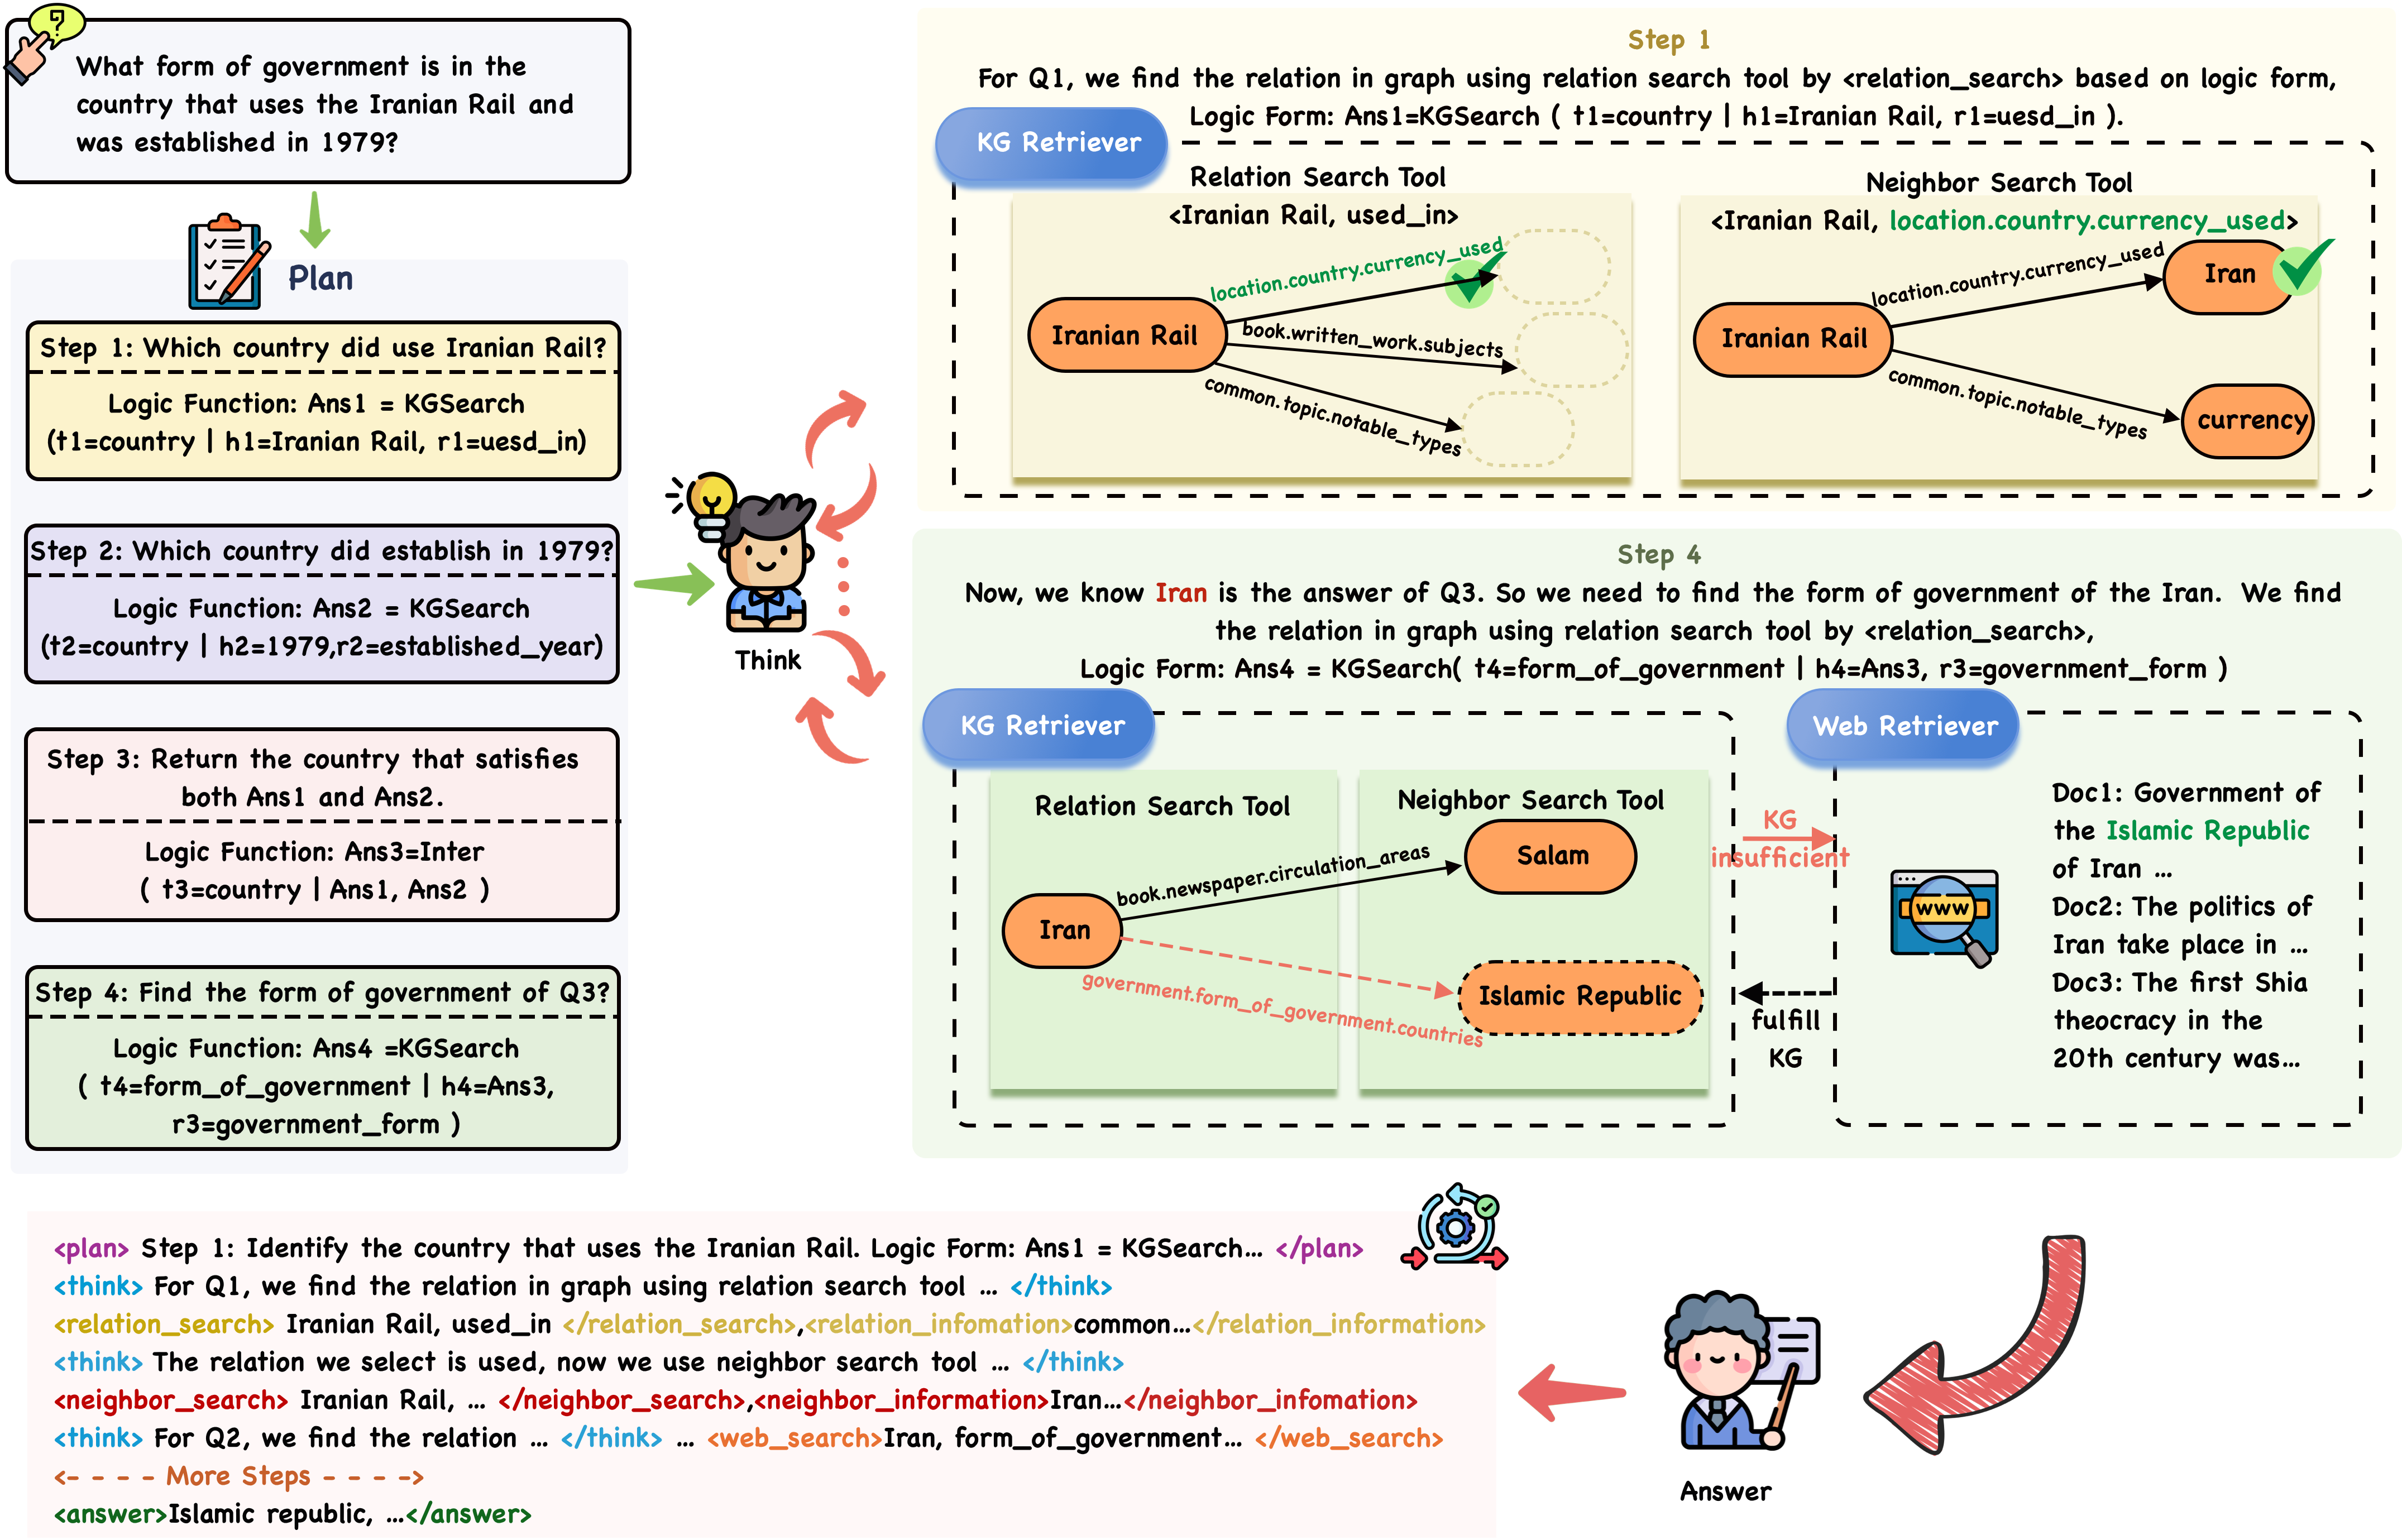
\includegraphics[width=.9\textwidth]{dataset_design.png}
    \caption{Graph-RFT Reasoning Trajectory for SFT dataset construction and rollout process for RL.}
    \label{fig:dataset}
    \vspace{-2ex}
\end{figure*}

% In the initial phase, we employ SFT on a structured reasoning dataset containing step-by-step planning, reasoning and retrieving processes. This phase trains the model to activate the model's planning-reasoning capability and establish robust cold start for downstream RL.
% The construction of our SFT dataset in Figure\ref{fig:dataset}, we monitor the process of planning and tool invocation process, recording the agent’s output by applying a multi-step interaction from KG and the search engine. This transforms the multi-step collaboration procedure into a CoT-like trajectory suitable for supervised fine-tuning. The annotation and filtering process of the dataset are in Appendix \ref{app:data_construct}. The training objective minimizes:
\vic{In the initial phase, we propose the CoT finetuning method using a structured reasoning dataset that contains step-by-step planning, reasoning, and retrieval processes. This phase is critical for activating the model's planning-reasoning capabilities and establishing a robust cold start for subsequent RL.
To construct our SFT dataset, as illustrated in Figure \ref{fig:dataset}, we monitor and record the agent's output throughout a multi-step interactive process with the KG and the external search engine. This approach transforms the complex, multi-step collaboration procedure into a  CoT-style trajectory suitable for SFT. In addition, we use a two-stage process to filter the trajectory to get the high quality dataset. The Details regarding the data's annotation and filtering processes are provided in \textcolor{blue}{Appendix \ref{app:data_construct}}. The training objective minimizes:}
\begin{equation}
    \mathcal{L}_{\text{SFT}} = - \sum_{t=1}^{T} \log \pi_{\theta}(y_t \mid q, y_{<t})
\end{equation}
\vic{where $q$ is the question, $y$ is the concatenated sequence of reasoning steps and the answer, $\pi_{\theta}$ is the model's token distribution.
The output model $\pi_{CoT}$ serves as the initialization for the next stage \cite{tan2025reason}, ensuring a robust foundation for RL.}

\subsection{RL-based Reasoning Enhancement}
\label{second_stage}
\subsubsection{Rollout with Search Tools}
\label{rollout}
% Our approach follows an iterative framework where the LLM alternates between text generation and external search engine queries. Specifically, our method consists of three steps: 
% i) Plan the procedure of sub-problem decomposition and tool invocation for complex reasoning in a specific order; 
% ii) Retrieve corresponding answers from the knowledge graph based on the priority and logic function of these subproblems;
% iii) Obtain the correct answers by searching external sources for information not available in the knowledge graph.

\vic{Our approach follows an iterative framework where the LLM alternates between text generation and external search engine queries. Specifically, our method consists of three steps: 
i) Plan the sub-problem decomposition and tool invocation for complex reasoning in a specific order; 
ii) Retrieve corresponding answers from the knowledge graph based on the priority and logical functions of these subproblems;
iii) Obtain the correct answers by searching external sources for information not available in the knowledge graph.}

\noindent \textbf{Plan the Steps.} 
\vic{We adhere to the Cartesian principle of breaking down complex problems into distinct steps, while designing logical functions to assist the model in understanding the interrelationships between sub-problems and determining the appropriate timing for tool utilization.
% , Descartes proposed four principles for solving problems scientifically: 1) Doubt every thing, avoiding precipitancy and prejudice. 2) Divide any complex question into multiple simpler subquestions. 3) Order sub-questions from the simplest to the most complex and fix them step by step. 4) Once all issues are solved, review them to ensure that nothing was omitted. 
In Figure \ref{fig:dataset}, the first two steps correspond to subproblems of higher priority, as they do not rely on answers from other subproblems. Additionally, we use logical functions to represent the parameters for invoking KG retrieval tool, which helps the model gain a clear understanding of the invocation process. Step 3 expresses the logical relationship between the two subproblems through the $\textit{inter}(Ans_1, Ans_2, .., Ans_n)$  function (the intersection of the answers to subquestions), passes the returned results to Step 4, and obtains the final answer by invoking the KG retrieval tool.
The planning steps are encapsulated between <plan> and </plan>.} 

\noindent \textbf{Retrieve Facts from the KG.} \vic{For each single steps obtained through planning, we need to sequentially select relevant triples from the KG. To address this, we design two interactive toolkits.}

\begin{itemize}[itemsep=0.5ex, leftmargin=3mm]
\item \textbf{Relation Search Tool.} \vic{This tool retrieves a set of candidate relations for an entity in a given single-hop problem. The LLM encapsulates the entity and the hypothetical relation from the logical function between the relation search tokens <relation\_search> and </relation\_search>. By invoking the relation acquisition toolkit, the set of top 15 relations that are similar to the hypothetical relation is encapsulated between the tokens <relation\_information> and </relation\_information>.}
\item \textbf{Neighbor Search Tool.} \vic{This tool retrieves the tail entity corresponding to a given head entity-relation  pair selected by LLMs. The LLM encapsulates the specified head entity and relation between the neighbor search tokens <neighbor\_search> and </neighbor\_search>. By invoking the neighbor acquisition toolkit, the answer is then encapsulated between the tokens <neighbor\_information> and </neighbor\_information>.}

\end{itemize}
% \vic{Given then obtained single-hop questions, e.g., "Identify the country that uses the Iranian Rail", we first invoke the Relation Search Tool to retrieve a candidate set of relations associated with the initial entity\nb{V: what is an initial entity?}. The LLM then reasons over this set and selects the most appropriate relation, e.g.,  select ``used'' to replace ``used\_in'' occurring in the original logical function\nb{what is the original logical function?}. This greedy strategy simplifies the reasoning process by choosing a locally optimal relation at each step, thereby reducing reliance on global information. Next, the Neighbor Search Tool is called to obtain the specific  triples and corresponding answers, e.g., ``The Islamic Republic of Iran''. If the LLMs determine that the retrieved triples are insufficient to answer the question, or if no answer is retrieved from KG, i.e.,  when <neighbor\_information> and </neighbor\_information> returns ``No information in the KG, please use web tool", proceed directly to use search engine. The answers to higher-priority\nb{V: I have seen that a couple of times priority is mentioned, but it is not clear how the priorities are established} single-hop questions can then be combined with those of lower-priority ones to generate new single-hop questions. By iteratively repeating this process, the system is able to derive answers to complex multi-hop questions. Notably, if the maximum iteration limit is reached without successfully generating an answer, the parametric knowledge of LLMs will be used to respond.}
\vic{Given the obtained single-hop questions (e.g., ``Identify the country that uses the Iranian Rail''), we first invoke the Relation Search Tool to retrieve a candidate set of relations associated with the initial (topic) entity. The LLM then reasons over this set and selects the most appropriate relation, for example, choosing ``location.country.currency\_used'' to replace ``used\_in'' in the retrieval function.
This greedy strategy simplifies the reasoning process by selecting a locally optimal relation at each step, thereby reducing reliance on global contextual information. Next, the Neighbor Search Tool is called to obtain specific triples and their corresponding answers (e.g., ``Iran'').
If the LLM determines that the retrieved triples are insufficient to answer the question, or if no answer is found in the knowledge graph (i.e., when <neighbor\_information> and </neighbor\_information> return “No information in the KG, please use web tool”), the system directly invokes the search engine.
The answers to higher-priority (according to the order produced by the subquestion plan)
%\nb{V: I have seen that a couple of times priority is mentioned, but it is not clear how the priorities are established}  \nb{\textcolor{red}{"Priorities" refers to the order of sub-problems within a plan. Sub-problems in Step 1 have higher priority and thus are placed first. Specifically, those "most basic ones that do not rely on any prior information" are given higher priority. As for how to establish such priorities, it follows the guideline in Cartesian principles: "Order sub-questions from the simplest to the most complex and fix them step by step."}} 
single-hop questions can then be combined with those of lower-priority ones to generate new single-hop questions. By iteratively repeating this process, the system is able to derive answers to complex multi-hop questions. Notably, if the maximum iteration limit is reached without successfully generating an answer, the parametric knowledge of the LLM is used to provide a final response.}
% \begin{figure*}[t!]
%     \centering
%     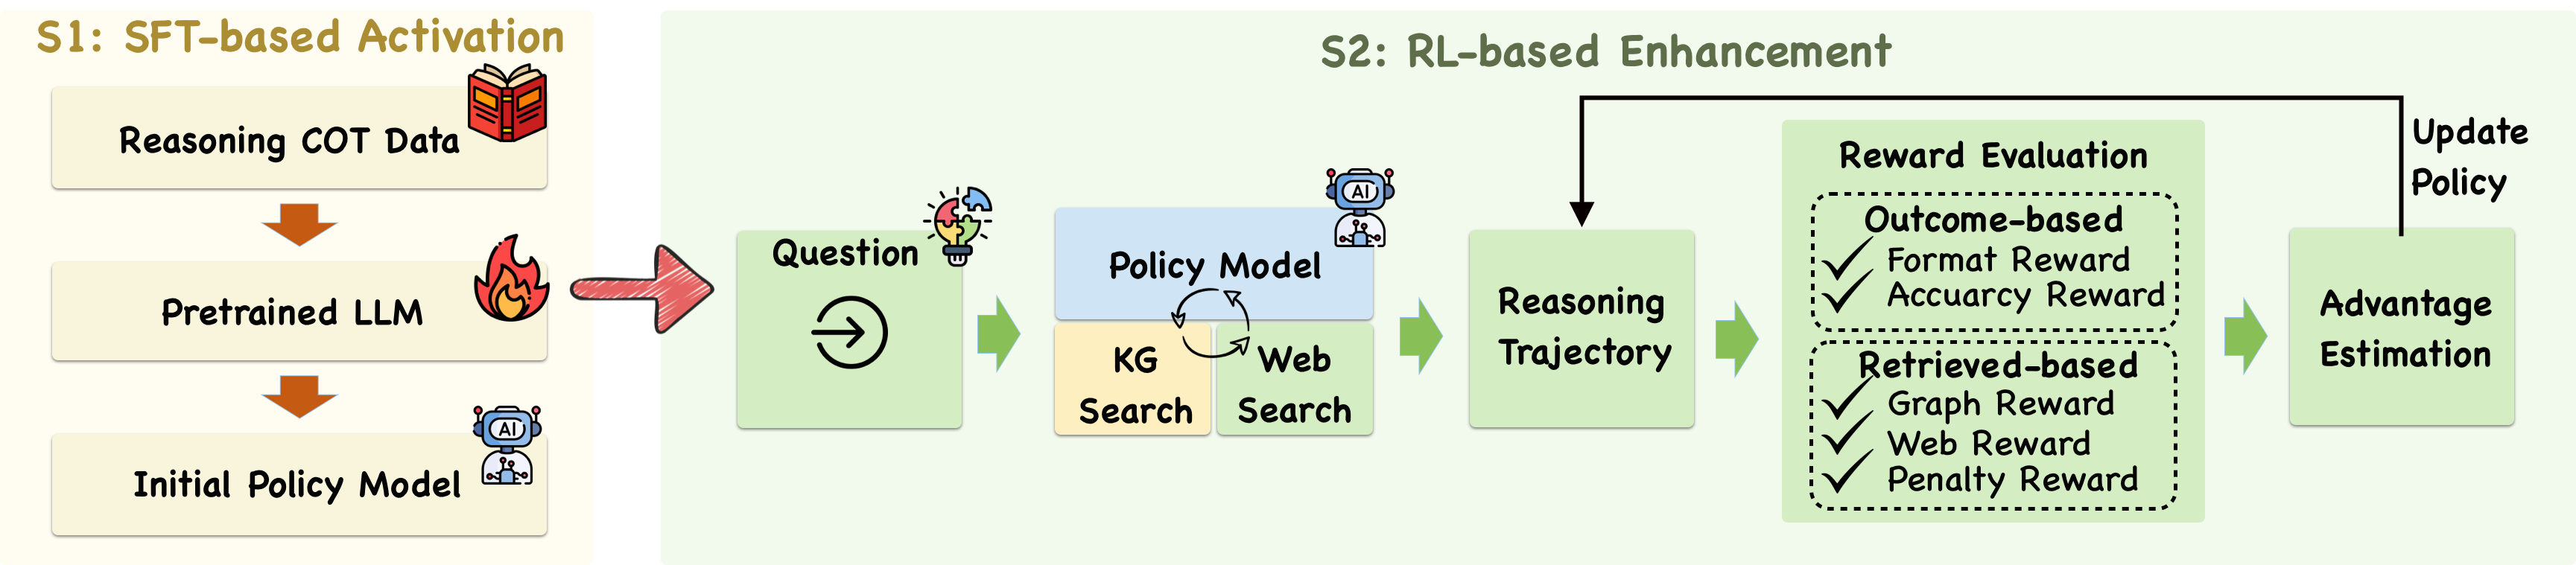
\includegraphics[width=.9\textwidth]{method.png}
%     \caption{Graph-RFT Training Framework: SFT-based Reasoning Activation (S1) and RL-based Reasoning Enhancement (S2).}
%     \label{frame}
%     \vspace{-2ex}
% \end{figure*}

% \noindent \textbf{Complete with Search Engine.} When LLMs think the knowledge retrieved by KG search tools is insufficient and unreasonable, or the KG lacks information (<neighbor\_information> and </neighbor\_information> returns "No information in KG, please use web tool."), the LLM encapsulates the head entity and relation, for which no information can be retrieved, within the special search tokens <web\_search> and </web\_search>. After that, a search engine is invoked, and the retrieved documents from Bing website are wrapped within <web\_information> and </web\_information>. This process not only enables the model to gather the necessary information to answer the question but also helps identify the missing factual triples, which can be used to augment the KG and therefore address the challenge of KG incompleteness. In our experiments, we fixed the TOP-K value (eg. 3) in order to control the number of retrieved documents.
\vic{When LLMs determine that the knowledge retrieved through KG search tools is insufficient or implausible (such as when the KG lacks relevant information, i.e., the tags <neighbor\_information> and </neighbor\_information> return ``No information in KG, please use web tool.''), the model encapsulates the corresponding head entity and relation, for which no information is available, within the special search tokens <web\_search> and </web\_search>. Subsequently, a search engine is invoked, and the documents retrieved from the Bing website are enclosed within <web\_information> and </web\_information>. This mechanism not only enables the model to acquire the supplementary knowledge required to answer the query but also facilitates the identification of missing  triples, which can later be incorporated into the KG to mitigate its incompleteness. In our experiments, we fixed the top-$k$ value (e.g., 3) to control the number of retrieved documents.
}
\subsubsection{Reward Design}
\label{rewards}
% In RL, the design of the reward function is crucial. Previous work has primarily relied on outcome-based rewards to guide LLMs in learning reasoning and search engine utilization throughout the entire reinforcement learning process. However, this form of supervision fails to fully explore different retrieval-related reward mechanisms and cannot effectively guide the retrieval process in incomplete KG. Therefore, we have integrated two fundamental components into our reward design: (i) outcome-based reward, which directly evaluates the answers generated by the model; and (ii) retrieval-specific reward, which encourages the model to identify how and when to extract relevant information from knowledge graphs or web documents.
\begin{sloppypar}
    To further optimize the above retrieval-planning process, we propose the GRPO \cite{shao2024deepseekmath} based RL method with the novel multi-reward design. Prior studies have predominantly employed outcome-based rewards to guide LLMs in developing reasoning abilities and leveraging search engines throughout the reinforcement learning process. However, such supervision alone does not sufficiently capture diverse retrieval-oriented reward mechanisms and is inadequate for effectively guiding retrieval in the presence of incomplete KGs. To address this limitation, we incorporate two key components into our reward design: (i) an outcome-based reward, which directly evaluates the quality of the model’s generated answers; and (ii) a retrieval-specific reward, which encourages the model to discern when and how to extract relevant information from knowledge graphs or web documents.
\end{sloppypar}

\begin{table*}[t]
\caption{Results of Graph-RFT across various datasets (represent the maximum hop), compared with the state-of-the-art (SOTA) in Supervised Learning (SL) and In-Context Learning (ICL) methods. The highest scores for ICL methods are highlighted in bold, while the second-best results are underlined. The Prior FT (Fine-tuned) SOTA includes the best-known results achieved through supervised learning. CKG denotes using complete knowledge graph and IKG denotes using incomplete KG (IKG-40\%).}
\label{fig:mainresult}
\small
\begin{tabular}{@{}ccccccccccc@{}}
\toprule
Method        & Class & LLM           & \multicolumn{6}{c}{Multi-Hop KGQA}   & \multicolumn{2}{c}{Single-Hop KGQA} \\ \cmidrule(lr){4-9}
              &       &               & \multicolumn{2}{c}{CWQ (4-hop)}  & \multicolumn{2}{c}{WebQSP (2-hop)}        & \multicolumn{2}{c}{GrailQA (4-hop)}       & \multicolumn{2}{c}{Simple Questions (1-hop)}    \\ \midrule
\multicolumn{11}{c}{\textit{Without external knowledge}}                                                                   \\\midrule
IO prompt\cite{sun2023think}     & -     & GPT-3.5-Turbo & \multicolumn{2}{c}{37.6} & \multicolumn{2}{c}{63.3}          & \multicolumn{2}{c}{29.4}          & \multicolumn{2}{c}{20.0}                      \\
CoT\cite{sun2023think}            & -     & GPT-3.5-Turbo & \multicolumn{2}{c}{38.8} & \multicolumn{2}{c}{62.2}          & \multicolumn{2}{c}{28.1}          & \multicolumn{2}{c}{20.3}                     \\
SC\cite{sun2023think}             & -     & GPT-3.5-Turbo & \multicolumn{2}{c}{45.4} & \multicolumn{2}{c}{61.1}          & \multicolumn{2}{c}{29.6}          & \multicolumn{2}{c}{18.9}                     \\ \midrule
 &       &               & CKG  & IKG  &  CKG & IKG       & CKG   & IKG       & CKG  & IKG   \\ \midrule
\multicolumn{11}{c}{\textit{With external knowledge}}                                                                      \\ \midrule
RoG  \cite{luo2023reasoning}  & SL    & Qwen2.5-7B-base        & 63.7 & 53.6 & 84.2 & 75.3        & -   & -     & -    & -           \\
ChatKBQA \cite{luo2023chatkbqa}  & SL     & Qwen2.5-7B-base      & 72.4  & 37.8 & 75.5      & 47.1    & -   & -     & -   & - \\ 
% Rule-KGQA \cite{zhang2025rule} &SL   & Llama-3-8B  & 73.5 & - & 84.1 & - & -   & -     & -    & -  \\
% KG-Agent\cite{jiang2024kg}  &SL   & -  & 72.2 & - & 83.3 & - & -   & -     & -    & -  \\
\midrule
KB-BINDER\cite{li2023few}     & ICL   & Codex         & -  & -  & 50.7 & 38.4          & -      & -    & -  & -                     \\
StructGPT\cite{jiang2023structgpt}     & ICL   & GPT-3.5-Turbo & - & - & 76.4    & 60.1      & -     & -     & -    & -  
\\
ToG/ToG-R\cite{sun2023think}     & ICL   & GPT-3.5-Turbo         & 47.2 & 37.9 & 76.9 & 63.4          & -    & -      & -    & -                  \\ 
% ToG-2.0\cite{ma2024think} & ICL   & GPT-3.5-Turbo  & - & - &81.1 &- & - & -   & -     & -    \\
ToG/ToG-R\cite{sun2023think}     & ICL   & GPT-4         & 71.0 & 56.1 & 80.3 & 71.8    & -  & -        & -    & -              \\ 
PoG\cite{tan2025paths}     & ICL   & GPT-4        & 76.8 & 62.6 & \textbf{96.7} & 76.4   & 79.2  & 64.1       & \textbf{80.2}   & \underline{59.5}            \\ 
% DoG\cite{ma2025debate} & ICL & GPT-3.5-Turbo        & 58.2 & - & 88.6 & -    & 77.8  & -        & -    & -  \\
% DoG\cite{ma2025debate} & ICL & GPT-4        & 56.0 & - & \textbf{91.0} & -    & 80.0  & -        & -    & -  \\
GoG\cite{xu2024generate}   & ICL   & GPT-3.5-Turbo         & 55.7 & 44.3 & 78.7  & 66.6         & 71.7  & 62.4        & 54.3   &  43.9                 \\ 
GoG\cite{xu2024generate}  & ICL   & GPT-4         & 75.2 & 60.4 & 84.4     & 80.3     & 76.8   & 69.4       & 68.9   & 56.4                \\ 
\midrule

Graph-RFT-instruct         &  RL  & Qwen2.5-7B-instruct & \underline{78.4}   & \underline{64.8}          &  87.3         & \underline{82.7} &\underline{82.1} &\underline{71.8} &73.8 & 58.7                \\
Graph-RFT-base         & RL   & Qwen2.5-7B-base &  \textbf{80.7}  &\textbf{67.2}           &   \underline{90.6}       &  \textbf{86.3} &\textbf{84.6} &\textbf{73.3} &\underline{76.9} &\textbf{62.4}                   \\ \bottomrule
\end{tabular}
\end{table*}

\noindent \textbf{Outcome-based Reward.}
\vic{Result-based reward are divided into format reward and answer reward. For format reward, we first define the correct format to ensure that the LLM adopts the predefined iterative workflow of "Think-Decompose-Retrieval-Search". The definitions of the model's thinking process, tool invocation, and final answer output format are shown in Figure \ref{fig:prompt} in \textcolor{blue}{Appendix \ref{app:prompt}}.
For answer rewards $r_{ans} \in [0, 1]$, we compare the predicted answer in  <answer></answer> with the ground-truth answer, and use the F1-score between the two sets as the reward to measure its accuracy. The complete accuracy reward $R_{acc}$ is defined as:}
\begin{equation}
    R_{\text{acc}} = 
\begin{cases} 
\max(0.1, r_{\text{ans}}), & \text{if format is correct}, \\
0, & \text{if format is incorrect}.
\end{cases} 
\end{equation}

\begin{equation}
r_{\text{ans}} = \text{F1}(p_{\text{ans}}, a) = \frac{2|p_{\text{ans}} \cap \{a\}|}{|p_{\text{ans}}| + |a|}
\end{equation}
%
\vic{where \( p_{\text{ans}} \) is the predicted answer, and \( a \) is the ground truth answer from the \((q, a)\) pair.}

\noindent \textbf{Retrieval-specific Reward.}
\vic{Inspired by AutoRefine~\cite{shi2025search}, building on the result-based reward described above, we further introduce two retrieval rewards to encourage LLMs to learn how to extract relevant information from both the KG and web documents. Specifically, we introduce a  graph retrieval reward $R_{graph}$ and a document search reward $R_{web}$. }

\begin{sloppypar}
\vic{$R_{graph}$ is measured based on the retrieval results contained in the <neighbor\_information></neighbor\_information> block. Specifically, we collect all graph retrieval results from the entire trajectory and concatenate them into a single text sequence:}
\begin{equation}
    \mathcal{R}_{\text{graph}} = \mathbb{I}\bigl(\{a\} \cap o_{\text{graph}} = a\bigr)
\end{equation}
\begin{equation}
    o_{\text{graph}} = \bigcup \left\{ c_t \mid (s_t, c_t) \in o \land s_t = \text{<neighbor\_information>} \right\}
\end{equation}

\vic{where $I(\cdot)$ is the indicator function, $o_{graph}$ is the concatenation of all the KG retrieval information steps.}
% \nb{V: above what is $o$? It needs to be clarified
% }.} \nb{\textcolor{red}{Sure! I have revised in Task Formulation:"Formally, for each question $q$, we generate a reasoning trajectory: $o = (\tau_1, \tau_2, . . . , \tau_T )$"}}

\vic{$R_{web}$ is defined in a similar way to $R_{graph}$. We collect all document retrieval results encapsulated in the <web\_information></web\_information> blocks throughout the entire trajectory and concatenate them into a single text sequence.}
\begin{equation}
    \mathcal{R}_{\text{web}} = \mathbb{I}\bigl(\{a\} \cap o_{\text{web}} = a\bigr)
\end{equation}
\begin{equation}
    o_{\text{web}} = \bigcup \left\{ c_t \mid (s_t, c_t) \in o \land s_t = \text{<web\_information>} \right\}
\end{equation}

\vic{where $I(\cdot)$ is the indicator function, $o_{graph}$ is the concatenation of all the web search information steps.} 
    
\vic{However, such multi-turn reinforcement learning is unstable. To prevent the model from bypassing graph retrieval and directly turning to document search in cases where the correct result could have been obtained through graph retrieval, we introduce a corresponding penalty for this behavior to help LLMs know when to use different retrieval tools. The overall reward $\mathcal R_{\text{over}}$ can be formally written as:}
\begin{small}
\begin{equation}
    \mathcal{R}_{\text{over}} = 
\begin{cases} 
\mathcal{R}_{\text{acc}}, & \text{if } \mathcal{R}_{\text{acc}} > 0, \\
0.1, & \text{if } \mathcal{R}_{\text{acc}} = 0 \text{ \& } \mathcal{R}_{\text{graph}} > 0   \text{ OR }     \mathcal{R}_{\text{acc}} = 0 \text{ \& }  \mathcal{R}_{\text{web}} > 0,\\
-0.1, & \text{if } \mathcal{R}_{\text{web}} > 0 \text{ when CKG} \text{ OR } \mathcal{R}_{\text{web}} = 0 \text{ when IKG}\\
0, & \text{if } \mathcal{R}_{\text{acc}} = \mathcal{R}_{\text{web}} = \mathcal{R}_{\text{graph}} = 0.
\end{cases}
\end{equation}
\end{small}
\end{sloppypar}

\noindent \textbf{Training Objective.}
% Combining the overall reward with the training objective of GRPO~\cite{shao2024deepseekmath}, we propose an RL objective that interacts with the KG and search engine during optimization for LLM search training. 
\vic{By integrating the overall reward with the GRPO training objective~\cite{shao2024deepseekmath}, our proposed learning objective enables dynamic interaction with both the knowledge graph and the search engine during optimization~\cite{jin2025search}, thereby facilitating effective LLM search training.
The objective is formalized as:}
\begin{equation}
\begin{split}
\max_{\pi_\theta} \mathbb{E}_{x \sim \mathcal{D}, \, y \sim \pi_\theta(\cdot | x; \mathcal{G},\mathcal{R})} \left[ r_\phi(x, y) \right] - \\ \beta \mathbb{D}_\text{KL} \left[ \pi_\theta(y | x; \mathcal{G},\mathcal{R}) \big\| \pi_\text{ref}(y | x; \mathcal{G},\mathcal{R}) \right]
\end{split}
\end{equation}
\vic{where $\pi_\theta$ denotes the trainable policy model, $\pi_\text{ref}$ is a fixed reference model, $r_\phi$ represents the overall reward function, and $\mathbb{D}_\text{KL}$ denotes the $KL$ divergence. Here, $x$ is sampled from the dataset $D$, and $y$ denotes the output sequence interleaving reasoning steps with KG and search engine retrievals. Since the retrieved triples and documents are not generated by the policy model, we mask the retrieval results during loss calculation to prevent the training policy from being biased \cite{hao2025dynasearcher}.}
%%
%% The acknowledgments section is defined using the "acks" environment
%% (and NOT an unnumbered section). This ensures the proper
%% identification of the section in the article metadata, and the
%% consistent spelling of the heading.

\section{Experiments}
% This section presents extensive experiments to evaluate Graph-RFT’s performance, focusing on four key questions: 
% \begin{itemize}
%     \item \textbf{Q1}: How does Graph-RFT perform compared to state-of-the-art (SOTA) baselines across various complex reasoning datasets?
%     \item \textbf{Q2}: What is the contribution of each key module in our Graph-RFT framework to the overall performance?
%     \item \textbf{Q3}: Can Graph-RFT effectively resolve information gaps through retrieval, especially under different degrees of KG incompleteness?
%     \item \textbf{Q4}: To what extent can Graph-RFT facilitate automatic KG completion?
% \end{itemize}
To evaluate the effectiveness of Graph-RFT, we aim to explore the following four research questions (RQs):
% \begin{itemize}[itemsep=0.5ex, leftmargin=3mm]
(1) \textbf{RQ1}: How does Graph-RFT perform against SOTA baselines on complex reasoning datasets?
(2) \textbf{RQ2}: What are the contributions of each  Graph-RFT module to overall performance?
(3) \textbf{RQ3}: Can Graph-RFT effectively bridge information gaps via retrieval under varying KG incompleteness?
(4) \textbf{RQ4}: What are the error types of Graph-RFT?

% \end{itemize}
\begin{sloppypar}
\vic{\noindent\textbf{$\blacktriangleright$ Datasets.} We evaluate Graph-RFT on four KGQA datasets, including three multi-hop datasets: CWQ~\citep{talmor2018web}, WebQSP~\citep{yih2016value}, GrailQA~\citep{gu2021beyond} and one single-hop dataset: SimpleQuestions~\citep{petrochuk1804simplequestions}. We consider two scenarios: Complete Knowledge Graph (CKG) and Incomplete Knowledge Graph (IKG). For CKG, we directly use the datasets provided by GoG~\citep{xu2024generate}. For IKG, since GoG only provides CWQ and WebQSP, we construct IKG versions of GrailQA and SimpleQuestions by sampling 3,000 multi-hop questions from GrailQA and 3,000 questions from SimpleQuestions. We further generate four IKGs with varying completeness levels IKG-20\%, IKG-40\%, IKG-60\%for example, IKG-40\% removes 40\% of the critical triples for each question and all relations between the corresponding entity pairs. Freebase~\citep{bollacker2008freebase} serves as the background KG for all datasets. 
The impact of using alternative knowledge graphs is discussed in \textcolor{blue}{Appendix~\ref{knowledege_bases}}.
}\\
\vic{\noindent\textbf{$\blacktriangleright$ Evaluation Metrics.} Following prior work~\cite{li2023chain, baek2023knowledge, jiang2023structgpt, sun2023think}, we adopt exact match accuracy (Hits@1) as the evaluation metric for all datasets.
%, consistent with prior studies \cite{li2023chain, baek2023knowledge, jiang2023structgpt, sun2023think}. 
Detailed descriptions of the baselines and implementation settings are provided in \textcolor{blue}{Appendix~\ref{app:baseline}} and \textcolor{blue}{Appendix~\ref{app:imp}}.
}
\end{sloppypar}

% \textbf{Datasets Details and Evaluation Metrics}
% \begin{sloppypar}
% We evaluate Graph-RFT on four KGQA datasets, including three multi-hop datasets (CWQ \cite{talmor2018web}, WebQSP \cite{yih2016value}, GrailQA \cite{gu2021beyond}) and one single-hop datasets (SimpleQuestions \cite{petrochuk1804simplequestions}). Note that for two large datasets, GrailQA and Simple Questions, we select 3,000 samples with 2 to 4 hops from GrailQA to ensure the complexity of the questions while saving computational costs. For Simple Questions, we randomly select 3,000 samples for testing. For each dataset, we generate four incomplete KGs with varying degrees of completeness based on GoG: IKG-40\%, representing randomly drop 40\% crucial triples for each question. In addition to the crucial triples themselves, all relations between these two entities will also be deleted. Moreover, Freebase \cite{bollacker2008freebase} servers as the background knowledge graph for all datasets. The discussion of different Knowledge bases impaction is in Appendix \ref{app:knowledge_base}. For all datasets, we use exact match accuracy (Hits@1) as our evaluation metric following previous works \cite{li2023chain, baek2023knowledge, jiang2023structgpt, sun2023think}. For the baselines and implementation detail can refer to Appendix \ref{app:baseline} and Appendix \ref{app:imp}. 
% \end{sloppypar}
% \subsection{Performance Comparison with SOTA}
\subsection{\zhiwei{Main Results (RQ1)}}

% This subsection compares (cf. Table \ref{fig:mainresult}) Graph-RFT with SOTA SL and ICL methods on four KGQA datasets (three multi-hop, one single-hop) under the incomplete (IKG) KG setting, using Hit@1 as the evaluation metric.
\vic{Table \ref{fig:mainresult} presents our main results on four KGQA datasets. We can observe that Graph-RFT consistently achieves SOTA performance across all settings in IKG, even when built upon smaller backbones such as Qwen2.5-7B-base, outperforming GPT-4-based methods.}
% From the results, we can observe that Graph-RFT-base achieves superior performance across all datasets under both complete and incomplete KG settings.

\noindent  $\blacktriangleright$ \textbf{CKG Setting.} Under the CKG setting, where all relevant triples are available, Graph-RFT achieves the strongest overall performance across both multi-hop and single-hop benchmarks. The results reveal that our two-stage RFT which combines CoT-based reasoning activation and plan–retrieval RL—provides consistent advantages over both prompt-only ICL methods and supervised learning baselines.
ICL approaches such as PoG and GoG rely purely on prompt engineering and lack any fine-tuning or reinforcement optimization. Although they perform competitively on simpler datasets such as WebQSP and SimpleQuestions, they struggle to generalize across long reasoning chains. In contrast, Graph-RFT-base (Qwen-2.5-7B) achieves substantial gains on complex benchmarks like CWQ (80.7 vs 76.8/75.2) and GrailQA (84.6 vs 79.2/76.8), where multi-step logical dependencies are required. These improvements highlight how explicit CoT supervision enables structured planning, and reinforcement optimization refines the timing and sequencing of retrieval actions.
Relative to RoG and ChatKBQA, which are purely supervised fine-tuned models, Graph-RFT demonstrates marked improvements (e.g., CWQ 80.7 vs 72.4/63.7, WebQSP 90.6 vs 84.2/75.5). This suggests that reinforcement learning contributes beyond imitation: by rewarding accurate retrieval scheduling and penalizing inefficient queries, the model learns to maintain global reasoning consistency and to balance exploration between relation-search and neighbor-search tools.
%\vic{Under the CKG setting, our model (particularly Qwen-2.5-7b-base) outperforms GoG with GPT-4 on all datasets. This advantage primarily comes from Graph-RFT’s planning, which decomposes a question into prioritized sub-questions, uses logical functions to plan the logic relation between different sub-questions and dynamically updates the lower-priority ones during the step-by-step retrieval process.}
%In addition, Graph-RFT-base outperforms PoG and GoG with GPT-4 in complex scenarios (e.g., CWQ, GrailQA) though PoG is more adept at handling simple problems.  GoG is constrained to local decision-making, lacking planning capabilities for question understanding and tool invocation and underscoring the effectiveness of our designed plan process.\vic{In addition, Graph-RFT-base surpasses PoG and GoG (even when equipped with GPT-4) in complex scenarios such as CWQ and GrailQA, although PoG demonstrates stronger performance on simpler tasks. GoG, by contrast, is limited to local decision-making and lacks effective planning mechanisms for question comprehension and tool invocation, further underscoring the effectiveness of our proposed planning process.}


\begin{table}[htbp]
\centering
\caption{Ablation study for the Graph-RFT-base in rollout framework.}
\resizebox{\linewidth}{!}{
\label{tab:ablation}
\begin{tabular}{l|ccc|cccc}
\toprule
&\textbf{PS} & \textbf{KR} & \textbf{WR}  & \multicolumn{3}{c}{\textbf{Multi-Hop KGQA}}   & \multicolumn{1}{c}{\textbf{Single-Hop KGQA}} \\ \cmidrule(lr){5-7}
 & &  &  & CWQ & WebQSP & GrailQA & Simple Questions \\
\midrule
 \textbf{Variants}& -& \checkmark& -  & 49.4 & 69.7 & 58.9 & 53.8 \\
  & - & \checkmark  &\checkmark  & 55.3 & 74.2 & 63.5 & \underline{61.7} \\
 & \checkmark &\checkmark  & - & \underline{62.6} & \underline{83.4} & \underline{69.1} & 57.3 \\ \midrule
\textbf{Graph-RFT-base} & \checkmark & \checkmark  & \checkmark & \textbf{67.2} & \textbf{86.3} & \textbf{73.3} & \textbf{62.4} \\
\bottomrule
\end{tabular}
}
\end{table}

\begin{table}[htbp]
\centering
\caption{Ablation analysis on Graph-RFT-base SFT and multi-reward design.}
\resizebox{\linewidth}{!}{
\label{tab:reward}
\begin{tabular}{l|cccc}
\toprule
Method & \multicolumn{3}{c}{\textbf{Multi-Hop KGQA}}   & \multicolumn{1}{c}{\textbf{Single-Hop KGQA}} \\ \cmidrule(lr){2-4}
   & CWQ   & WebQSP   & GrailQA & Simple Questions \\
\midrule
Graph-RFT-base w/o SFT  &46.4&74.2& 56.4 &54.7 \\
Graph-RFT-base w/o $R_{web}$ & 66.3 & 83.5  &72.1 & 60.8 \\
Graph-RFT-base w/o $R_{graph}$ & 65.8& 82.7 & 71.6 & 61.6\\ \midrule
\textbf{Graph-RFT-base} & \textbf{67.2} & \textbf{86.3}  & \textbf{73.3} & \textbf{62.4}\\
\bottomrule
\end{tabular}
}
\end{table}

 \noindent $\blacktriangleright$   \textbf{IKG Setting.} 
 %Under the IKG setting, for SL methods, with Qwen2.5-7B-base as the backbone, our model outperforms both RoG and ChatKBQA. This is because these finetuned methods cannot directly interact with the KG, preventing them from identifying which triples are missing. For ICL methods, ToG, PoG and GoG deliver weaker results than Graph-RFT. 
% The reason is that when triples are missing from the KG, unlike these models, Graph-RFT can detect the gaps, retrieve relevant documents via a search engine, and complete the missing parts. %Other models, however, can only rely on the inherent knowledge stored in the LLM to answer. 
% On the other hand, thanks to its planning capabilities, unlike these models, Graph-RFT can proactively choose not to use a search engine when the triples in KG is sufficient, avoiding the introduction of noisy documents and can also learn the ability to invoke different external tools during the planning process. %However, other models may generate answers based on LLM's inherent knowledge due to the lack of global planning, tend to make misjudgments and fail to obtain answers that could have been directly retrieved from KG.
When the knowledge graph is incomplete, the benefits of Graph-RFT become even more pronounced. 
Prompt-based ICL approaches such as PoG and GoG (GPT-4) achieve competitive accuracy under complete KGs but degrade significantly once KG coverage is reduced. For example, GoG’s performance drops 7-15 points across CWQ (75.2→60.4) and GrailQA (76.8→69.4), while PoG falls from 76.8→62.6 on CWQ. These methods rely on static prompt patterns and local reasoning, lacking mechanisms to assess KG sufficiency or to seek supplementary evidence.
In contrast, Graph-RFT-base (Qwen2.5-7B) remains stable across both settings, outperforms among ICL methods. This resilience arises from our two-stage RFT: CoT fine-tuning teaches explicit question decomposition, and reinforcement optimization learns when and how to invoke external retrievals.
SL methods such as RoG and ChatKBQA also decline sharply under IKG (e.g., CWQ: 63.7→53.6; ChatKBQA: 72.4→37.8), as their fixed fine-tuning lacks interactivity with retrieval tools. In contrast, Graph-RFT maintains high accuracy (e.g., CWQ 67.2, WebQSP 86.3), confirming that reinforcement-based retrieval scheduling effectively compensates for missing triples through controlled web augmentation.
Moreover, Graph-RFT with Qwen2.5-7b-base outperforms methods without external knowledge (e.g., IO, CoT, SC prompting), demonstrating that KGs play a crucial role in reasoning tasks.
%\vic{When the knowledge graph is incomplete, the benefits of Graph-RFT become even more pronounced. Under the IKG setting, using Qwen2.5-7B-base as the backbone, our model outperforms both RoG and ChatKBQA among supervised learning (SL) methods. This improvement arises because these finetuned models are unable to directly interact with the KG, limiting their ability to identify missing triples. For in-context learning (ICL) methods, ToG, PoG, and GoG exhibit weaker performance compared to Graph-RFT. The key advantage of Graph-RFT lies in its capacity to detect missing triples within the KG, retrieve relevant information through a search engine, and thereby complete the missing knowledge.Moreover, owing to its planning capability, Graph-RFT can also determine when the KG provides sufficient information and proactively avoid unnecessary search operations, thus preventing the introduction of noisy documents. During this planning process, the model additionally learns to invoke different external tools adaptively and effectively.} \vic{By comparing the performance of Graph-RFT across different datasets, we observe that it consistently delivers superior results on both single-hop and multi-hop datasets. Under the IKG setting, compared with GoG powered by GPT-4, our model achieves relevant improvements of 11.3\%, 7.5\%, and 5.6\% on CWQ, WebQSP, and GrailQA, respectively. Notably, the best performance gain is observed on the more challenging CWQ dataset, highlighting the model’s ability to handle complex reasoning. For the single-hop dataset, Graph-RFT achieves a 10.6\% improvement on SimpleQuestions. Moreover, Graph-RFT with Qwen2.5-7b-base outperforms methods without external knowledge (e.g., IO, CoT, SC prompting), demonstrating that graphs play a crucial role in reasoning tasks.}

% \subsection{Ablation Study}
\subsection{\zhiwei{Ablation Studies (RQ2)}}

% We conduct the ablation study on the key components of Graph-RFT. Specifically, we divide the study into two parts to investigate the impacts of the rollout framework and multi-reward on Graph-RFT.

\zhiwei{We perform ablation studies to analyze the contributions of Graph-RFT’s key components. Specifically, we examine the effects of the rollout framework, SFT and the multi-reward mechanism in the RL stage.}\\
% \textbf{Exploration on rollout framework.}
% In this section, we investigate whether the Planning Steps Module (PS), KG Retrieval Module (KR), and Web Search Module (WR) within the rollout framework can enhance the performance of Graph-RFT when the knowledge graph (KG) is incomplete. 
% In Figure \ref{tab:ablation}, we construct model variants by removing these components and demonstrate that the absence of any single component significantly impairs the model's performance under the IKG-40\% setting. 
% Comparing PS+KR, KR+WR and KR alone, we observe that the PS+KR achieves better performance in multi-hop datasets, which indicates that planning global steps, including question decomposition with logic functions and tool invocation, is more valuable than blindly supplementing missing knowledge, demonstrating the validity of the PS module. 
% % Specifically, we argue that planning steps on decomposing questions with logic functions is of crucial importance. By comparing the experimental results of PS+KR with those of KR+WR and KR alone, it is proven that the "prioritized sub-question decomposition and step-by-step solving" pattern guided by the PS module is distinctly superior to the approach of directly searching for answers solely based on the original question. 
% In contrast, for single-hop dataset, we observe that KR+WR is higher than PS+KR, possibly because acquiring knowledge from external documents is more important than conducting global planning, verifying that Graph-RFT can effectively deal with complex problems.
% In addition, comparing the setting of KR+WR and KR alone, it is confirmed that combining structured knowledge (e.g., KG) with unstructured knowledge (e.g., web documents) has achieved significant improvements. 
% In conclusion, each of the aforementioned modules plays a unique and critical role, and collectively enhances the overall performance of the model when handling complex reasoning tasks.
\zhiwei{\noindent\textbf{$\blacktriangleright$ Exploration on Rollout Framework.} We analyze the contributions of the Planning Steps (PS), KG Retrieval (KR), and Web Retrieval (WR) modules within the rollout framework to Graph-RFT’s performance under the IKG-40\% setting. Figure~\ref{tab:ablation} presents model variants obtained by ablating these components, revealing that removing any single module substantially reduces performance. Comparing PS+KR, KR+WR, and KR alone, we observe that PS+KR achieves superior performance on multi-hop datasets, indicating that global planning—including question decomposition with logical operators and tool invocation—provides greater benefit than merely supplementing missing knowledge, thereby validating the effectiveness of the PS module. In contrast, on the single-hop dataset, KR+WR outperforms PS+KR, suggesting that leveraging external unstructured knowledge becomes more critical than global planning for simpler queries, which demonstrates Graph-RFT’s adaptability across tasks of varying complexity. Furthermore, the comparison between KR+WR and KR alone confirms that integrating structured knowledge from the KG with unstructured knowledge from web documents produces substantial improvements. Collectively, these results indicate that each module contributes uniquely, and their synergistic combination significantly enhances the model’s capability for complex reasoning tasks.
}
\begin{figure}[t]
  \centering
  \begin{tabular}{@{}cc@{}}
    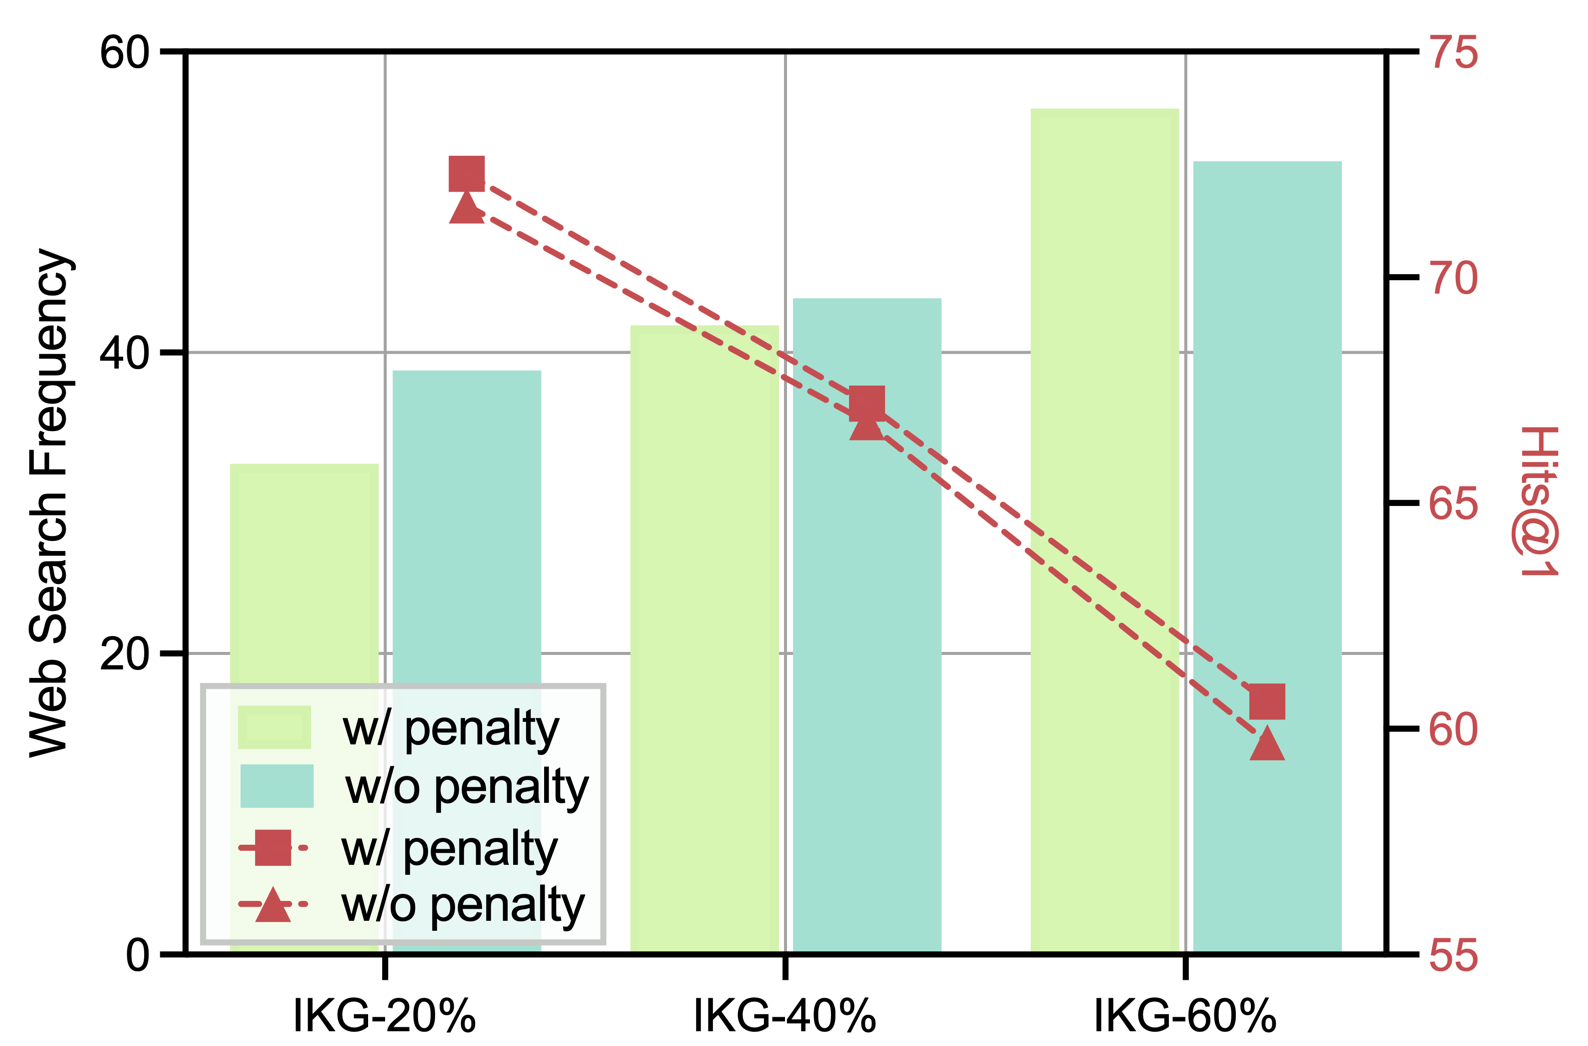
\includegraphics[width=.5\linewidth]{cwq_search.png} &
    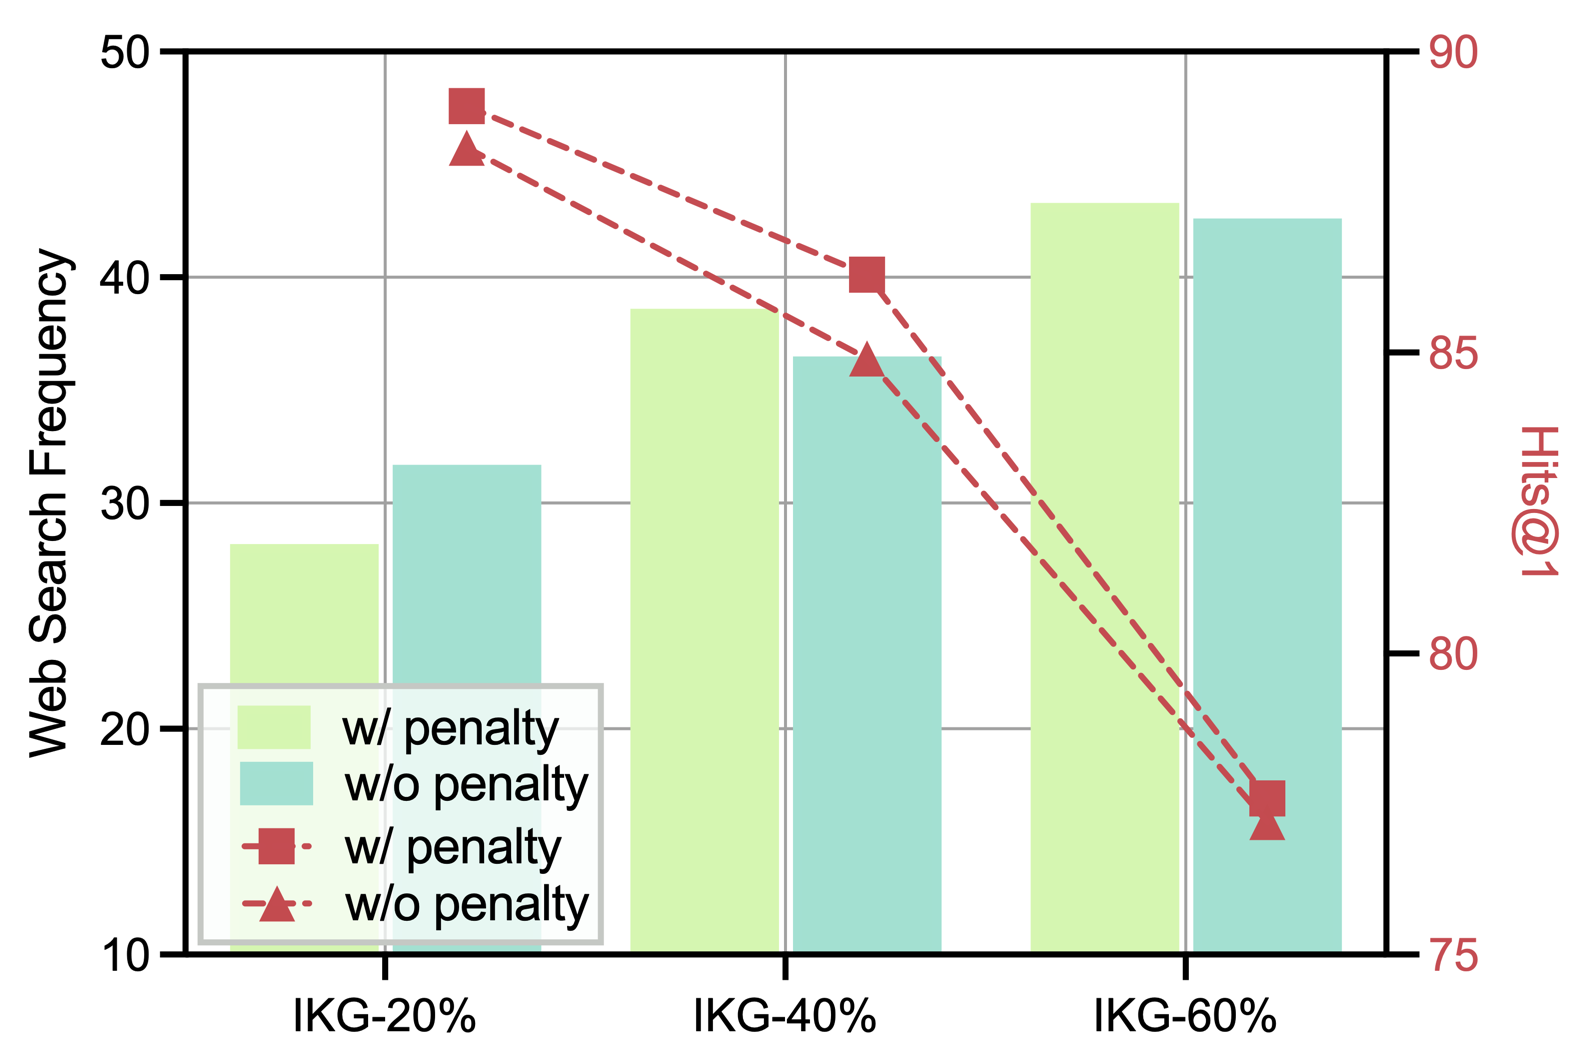
\includegraphics[width=.5\linewidth]{webqsp_search.png}
    \\
    \textbf{(a) CWQ.} &
    \textbf{(b) WebQSP.}
  \end{tabular}
  \caption{Ratio of web search operation in different KG settings under rewards with penalty or not.}
  \label{fig:exp2}
\end{figure}
\begin{figure}[t]
  \centering
  \begin{tabular}{@{}cc@{}}
    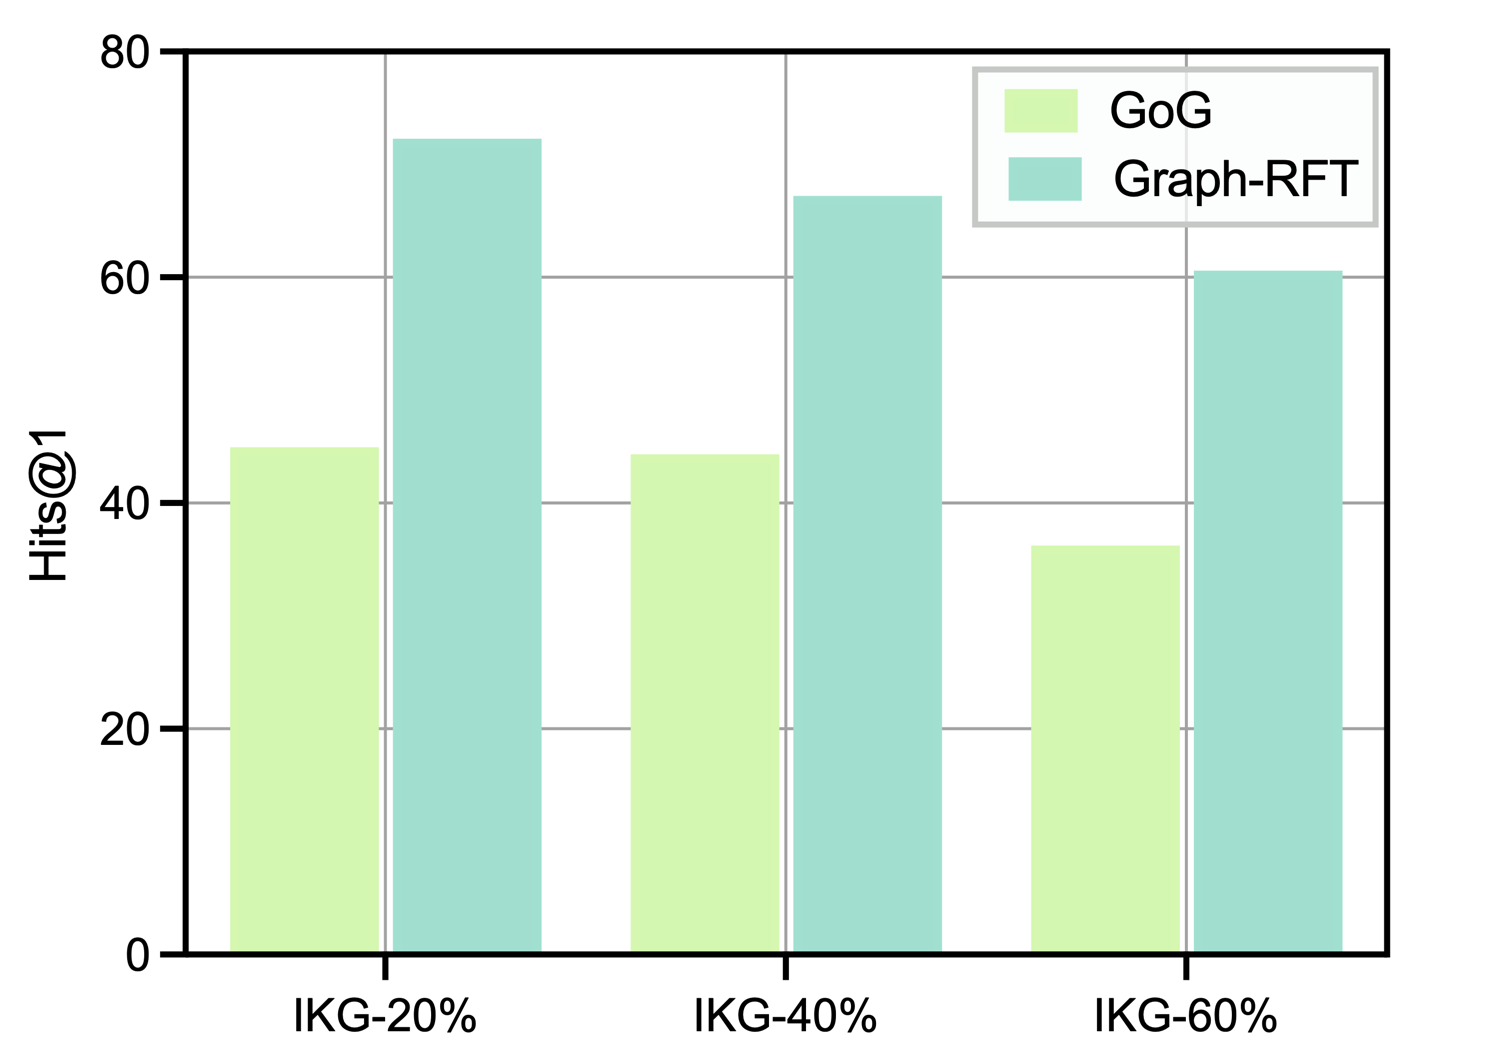
\includegraphics[width=.5\linewidth]{cwq_compare.png} &
    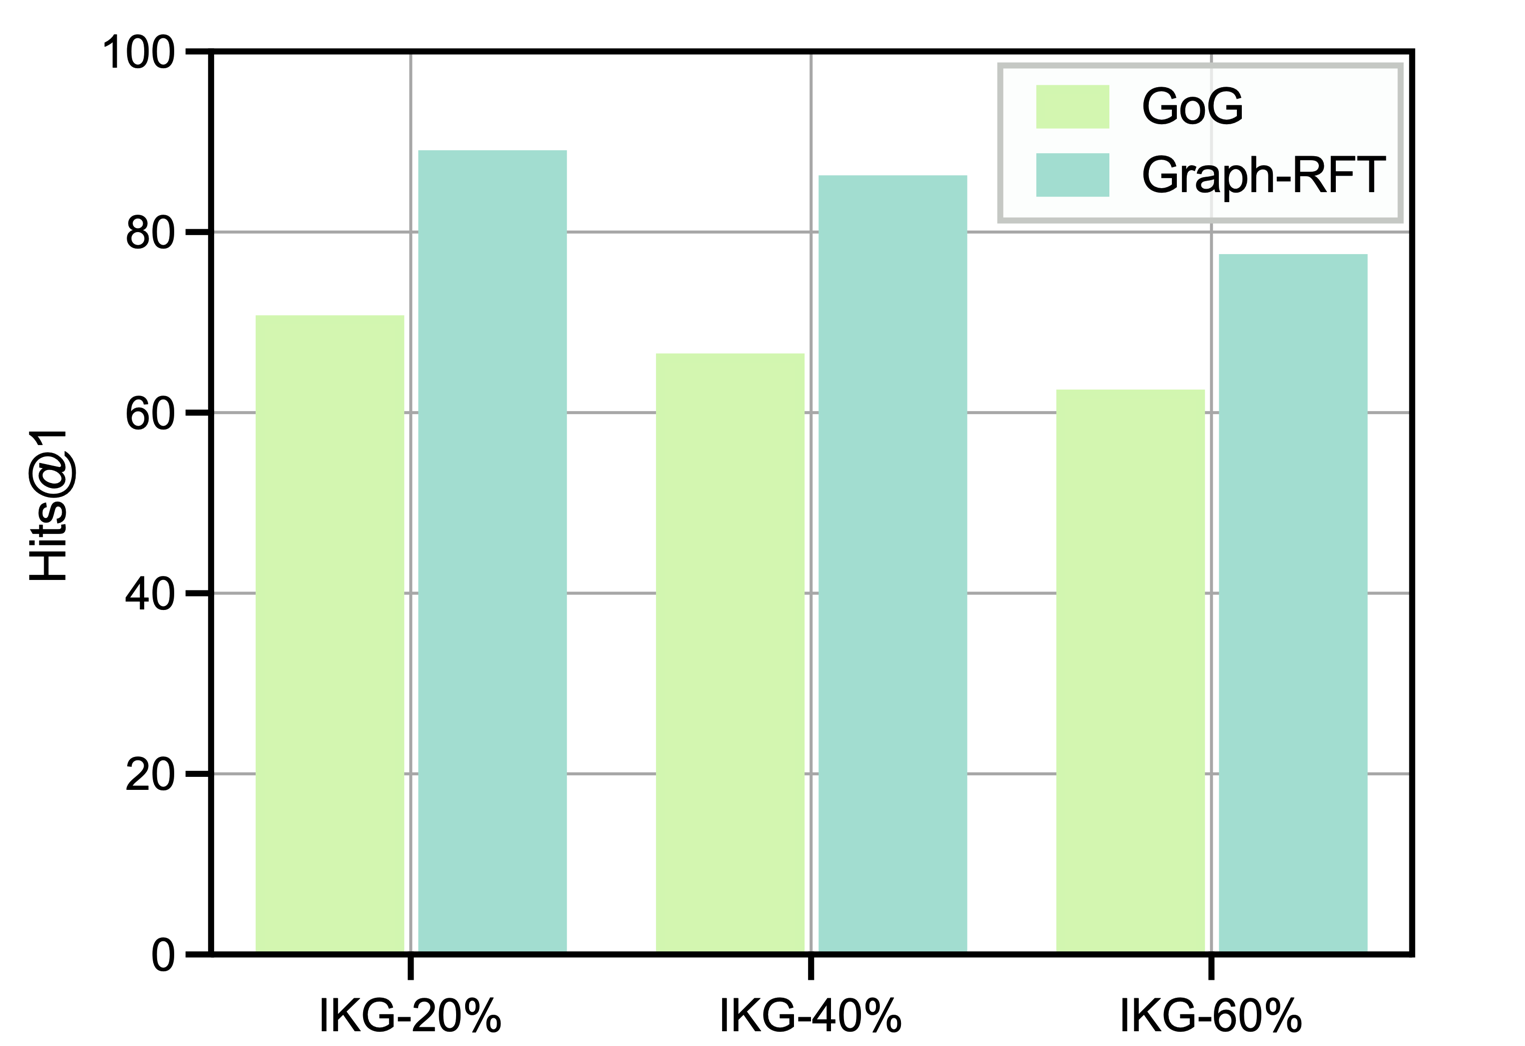
\includegraphics[width=.5\linewidth]{webqsp_compare.png}
    \\
    \textbf{(a) CWQ.} &
    \textbf{(b) WebQSP.}
  \end{tabular}
  \caption{Performance of GoG and our model under different KG settings.}
  \label{fig:compare}
\end{figure}
% \begin{figure*}[t!]
%     \centering
%     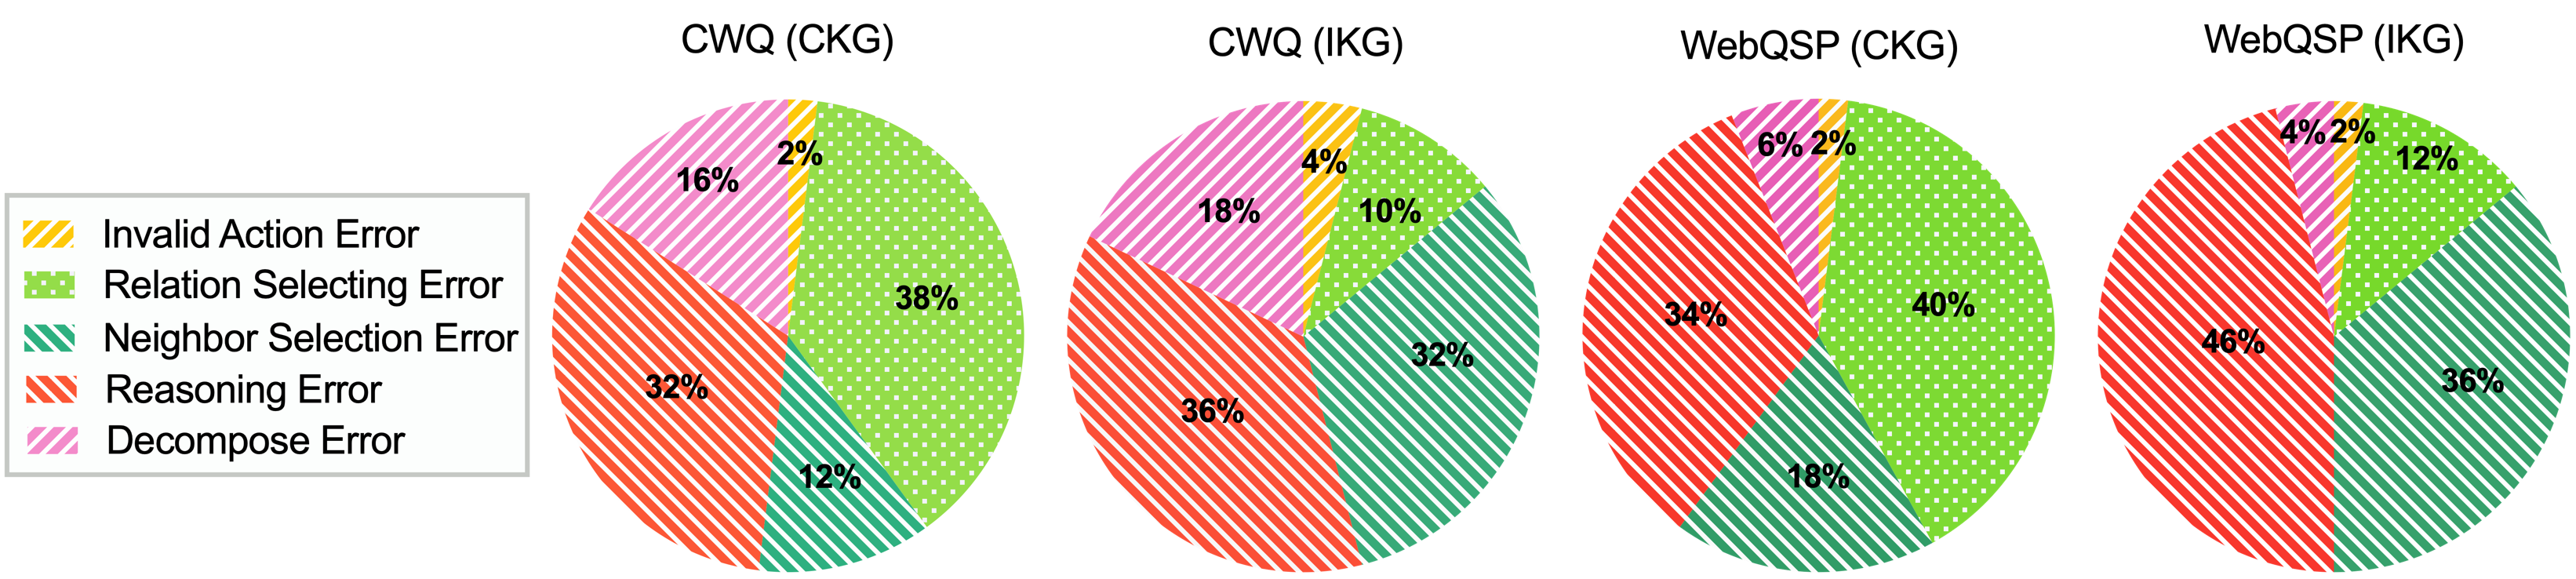
\includegraphics[width=.8\textwidth]{error_type.png}
%     \caption{Error Type}
%     \label{fig:error}
%     \vspace{-2ex}
% \end{figure*}
\\\zhiwei{\noindent\textbf{$\blacktriangleright$ Exploration on SFT and Multi-reward Design.} We further examine the effect of the SFT stage and the multi-reward mechanism on Graph-RFT’s performance under the IKG-40\% setting. Comparing Graph-RFT-base w/o SFT with Graph-RFT-base shows a marked performance drop across all datasets, underscoring the crucial role of SFT in strengthening model capability. Moreover, removing either the web retrieval reward or the graph retrieval reward consistently degrades performance, demonstrating that both rewards effectively guide the LLM to retrieve more semantically relevant triples and external documents. As shown in Figure~\ref{fig:exp2}, when the model’s web search frequency approaches the optimal level (e.g., 20\% in the IKG-20\% setting), performance on CWQ and WebQSP improves. This indicates that Graph-RFT can adaptively regulate web search frequency based on the sufficiency of KG information, reducing the risk of noisy or irrelevant content and thereby enhancing overall effectiveness.
}
% \textbf{Exploration on SFT and multi-reward design.}
% In this section, we investigate whether SFT stage and multi-reward improve the performance of Graph-RFT in incomplete KG (IKG-40\% setting). 
% Comparing Graph-RFT-base w/o SFT and Graph-RFT-base, there is a significant drop in all datasets, highlight the importance of SFT part. 
% Comparing Graph-RFT-base without web reward and graph reward, the results are all reduced, demonstrating that both web retrieval reward and graph retrieval reward can improve the retrieval process itself by guiding the LLM to retrieve more relevant triples and documents from the knowledge graph and external network.
% Furthermore, as shown in Figure \ref{fig:exp2}, for the penalty reward, when the frequency of web search called by the model approaches the correct value (IKG-20\% means the correct frequency is 20\%), the model's performance becomes better in CWQ and WebQSP. This indicates that our model can adaptively adjust the frequency of web searches based on the sufficiency of KG information, avoiding the introduction of noisy documents that would otherwise impair the performance.


% \subsection{Behaviors on different degrees of KG incompleteness}
\subsection{\zhiwei{Different KG Incompleteness (RQ3)}}
\label{exp2}
% The key capabilities of graph reasoning models are reflected in two aspects: (1) global planning for complex problems to fully utilize the knowledge within the KG; (2) identifying knowledge gaps that the KG itself cannot contain through web search. To evaluate these two core capabilities, we analyzed the performance of the Graph-RFT under different degrees of KG incompleteness and simultaneously counted its external search frequency. The relevant analysis results are shown in Figure \ref{fig:exp2}.

\zhiwei{The key capabilities of our model lies in performing global planning on complex problems to leverage the knowledge within the KG and identifying knowledge gaps beyond the KG through web search. We examine the performance of Graph-RFT under varying degrees of KG incompleteness and record its external search frequency, as shown in Figure~\ref{fig:exp2}. To evaluate the robustness of different methods under KG incompleteness, we compare GoG and Graph-RFT across KGs with different completeness levels, as illustrated in Figure~\ref{fig:compare}.
}\\ 
\zhiwei{\noindent\textbf{$\blacktriangleright$ Impact of Rewards with or without Penalty.} From Figure~\ref{fig:exp2}, Graph-RFT increases the frequency of external searches as KG completeness decreases. This behavior reflects the model’s ability to proactively compensate for missing knowledge required for reasoning through web retrieval. Moreover, the model’s search strategy varies notably with question complexity: compared to WebQSP (maximum 2-hop), Graph-RFT conducts significantly more external searches when tackling the more complex multi-hop questions in CWQ (maximum 4-hop). This demonstrates that the model can dynamically adjust its web search frequency according to question complexity, effectively aligning knowledge acquisition with the reasoning demands of the task. }\\
\zhiwei{\noindent\textbf{$\blacktriangleright$ Impact of Different KG Incompleteness.} From Figure~\ref{fig:compare}, we observe that Graph-RFT outperforms GoG across all degrees of incompleteness. This improvement arises because GoG is primarily confined to local decision-making, lacking the global planning needed for effective question understanding and tool invocation in complex problem decomposition. In contrast, when KG triples are missing, GoG relies solely on the LLM’s internal knowledge to generate answers, whereas our model retrieves relevant external documents through web search, thereby supplementing incomplete KG information and improving answer accuracy. Notably, the improvement on CWQ is much more pronounced than on WebQSP, validating Graph-RFT’s strong planning ability and logical decomposition mechanism for tackling complex reasoning tasks.}

% To investigate how different degrees of KG incompleteness affect different methods, we evaluate the performance of GoG (w/ GPT-3.5) under KGs with varying degrees of incompleteness, the results are demonstrated in Figure \ref{fig:compare}. It can be found that our Graph-RFT outperforms GoG in different degrees of incompleteness. This is because GoG is largely restricted to local decision-making instead of implementing global and hierarchical planning for the question understanding and tool invocation when decomposing complex problems. On the other hand, when triples are missing from the KG, GoG can only rely on LLM’s inherent knowledge to generate answers, whereas our model retrieves relevant documents via search engines, and supplements the missing information to boost answer accuracy.
% On the two datasets, our proposed Graph-RFT achieves a significant improvement in the Hits@1 score, and it fully underscores the importance of integrating incomplete structured KG with external unstructured knowledge and leveraging the reasoning capabilities of LLMs.
% Notably, the model's improvement on the CWQ is significantly greater than that on the WebQSP. This validates Graph-RFT's planning ability with logic functions for complex problem decomposition and tool invocation, fully utilizing the knowledge within KGs.

% Furthermore, although most of the questions in WebQSP are single-hop questions, Graph-RFT still outperforms the GoG model. This demonstrates that in addition to its excellent ability to decompose complex problems, Graph-RFT can also capture knowledge not covered by KGs from external resources; in contrast, the GoG model can only rely on the internal knowledge inherent to LLMs.

% Under the setting where KGs are incomplete, as shown in Figure \ref{fig:exp2}, when the completeness of the KG decreases, the Graph-RFT model invokes external searches more frequently. This is because when the KG lacks key knowledge required for reasoning, the model proactively supplements such gaps through web searches. 
% % This phenomenon reflects two core capabilities of Graph-RFT: first, a deep understanding of global planning for complex reasoning tasks; second, the ability to judge whether "the existing information in the KG is sufficient to support reasoning" and then decide whether to perform an external search accordingly. 
% Furthermore, the model’s search strategy exhibits significant differences when dealing with questions of varying complexity: compared to WebQSP (maximum 2 hop), Graph-RFT significantly increases the frequency of external knowledge searches when handling the more complex multi-hop questions in CWQ (maximum 4 hop). This demonstrates that the model can dynamically adjust the frequency of web search calls based on the complexity of the question, so as to match the knowledge requirements during the reasoning process.


% \subsection{Error Type Analysis}
\subsection{\zhiwei{Error Type Analysis (RQ4)}}
\zhiwei{To analyze Graph-RFT’s limitations, we randomly selected 50 failure cases from CWQ and WebQSP under both CKG and IKG settings. These cases are categorized into five types: (1) invalid actions, (2) relation selection errors, (3) neighbor selection errors, (4) reasoning errors, and (5) decomposition errors, with their distribution shown in Figure~\ref{fig:error}. We can obtain the following findings: (\textit{i}): reasoning errors—where the LLM follows a correct reasoning process but produces incorrect answers—represent the largest proportion in both datasets and are more prevalent in IKG than in CKG, likely due to answer aliasing and discrepancies between retrieved document answers and reference answers. (\textit{ii}): neighbor selection errors manifest in two scenarios: on the one hand, when relation selection is correct, neighbor errors are relatively rare in CKG, indicating that the model primarily struggles with relation selection; on the other hand, when the correct relation is not identified, as in IKG, the model often fails to determine whether entities are sufficient for problem-solving, resulting in incorrect neighbor selection. (\textit{iii}): decomposition errors, arising from flawed planning, occur more frequently on complex problems such as CWQ, whereas invalid action errors (e.g., invoking undefined tools) are effectively managed by the model. The case study is in \textcolor{blue}{Appendix \ref{case_study}}}.

% To gain a deeper understanding of the model's performance,as shown in Figure \ref{fig:error} 
% we categorized the failure cases into four types: 1) Invalid actions, where the model invokes actions not defined in the operational toolset; 2) Relation selection errors, where the LLM fails to understand the question or does not return relations related to the entity, making it difficult for the LLM to select the most relevant relation; 3) Decomposition errors, where the LLM forgets the original question after multiple rounds of retrieval and answers incorrect sub-questions; 4) Answer aliasing errors, where the LLM provides an alias of the ground truth. 

% To analyze Graph-RFT’s deficiencies, 50 failure cases were randomly selected from CWQ and WebQSP under CKG and IKG settings. These cases were categorized into five types: 1) Invalid actions, 2) Relation selection error, 3) Neighbor selection error, 4) Reasoning errors, 5) Decomposition errors (see Figure \ref{fig:error} for distribution).
% Reasoning errors (LLM with correct reasoning process but wrong answers) account for the largest proportion in both datasets, and are more common in IKG than CKG—likely due to answer aliasing and discrepancies between searched document answers and reference answers in IKG.
% Neighbor selection errors have two scenarios: 1) Errors occur when relation selection is correct. In CKG, relation selection errors are far more frequent than neighbor errors, indicating the model tends to choose incorrect relations. 2) Errors occur when the correct relation is not found. In IKG, the model often failed to judge if entities are sufficient for problem-solving, leading to wrong neighbor selection.
% Decomposition errors (caused by flawed planning) are more frequent in more complex problems (CWQ). Invalid action errors (calling undefined tools) were well-handled by the model.

% To analyze the deficiency of Graph-RFT, we randomly select 50 failure cases from CWQ and WebQSP under CKG and IKG settings. Figure \ref{fig:error} shows the distribution of these failure cases. In practice, most errors stem from relation selection errors and answer aliasing errors. Furthermore, under the IKG setting, answer aliasing errors are generally more common than those under the CKG setting. This is because there are discrepancies between the answers from the searched documents and the reference answers.

\section{Conclusion}
We introduced Graph-RFT, a two-stage reinforcement fine-tuning framework for complex reasoning over incomplete knowledge graphs. Graph-RFT unifies structured planning and adaptive retrieval within a single learning paradigm, enabling LLMs to reason coherently and retrieve information dynamically across KGs and web sources.
In the first stage, a CoT fine-tuning process with a customized plan–retrieval dataset activates the model’s planning and reasoning capabilities while mitigating the GRPO cold-start problem. In the second stage, a plan–retrieval guided reinforcement learning procedure with a multi-reward design optimizes coverage-aware retrieval scheduling and multi-step logical consistency.
Extensive experiments across multiple KGQA benchmarks demonstrate that Graph-RFT consistently outperforms strong baselines, achieving superior accuracy even with smaller LLM backbones.
In the future, we will explore enhancing relation
filtering performance from KGs and the capability of decomposing problems when dealing with complex reasoning tasks.
%\vic{In this paper, we introduce Graph-RFT, a novel two-stage reinforcement fine-tuning framework for complex reasoning over incomplete knowledge graphs. In the SFT stage, we design a high-quality CoT trajectory dataset to activate Graph-RFT's planning and reasoning capabilities. In the RL stage, we propose a multi-reward framework to  invoke tools interacting with plan steps via RL to address the incompleteness issue of KGs.Extensive experiments demonstrate the superiority of Graph-RFT, showcasing the potential to foster mutual enhancement between KG and LLM. In the future, we will explore enhancing relationfiltering performance from KGs and the capability of decomposing problems when dealing with complex reasoning tasks}.

\begin{acks}
We thank all anonymous reviewers and area chairs for their comments. This work is supported by the National Natural Science Foundation of China (U23A20316), the CCF-Tencent Rhino-Bird Open Research Fund (CCF-Tencent RAGR20250115), and the computing power resources from Wuhan Dongxihu District Intelligent Computing Center.
% We would like to thank all the anonymous reviewers and area chairs for their comments. This research is supported by the National
% Natural Science Foundation of China (U23A20316) and CCF-Tencent Rhino-Bird Open Research Fund (CCF-Tencent RAGR20250115). Our research is supported by the computing power resources of the Wuhan Dongxihu District Intelligent Computing Center.
\end{acks}

%%
%% The next two lines define the bibliography style to be used, and
%% the bibliography file.
\bibliographystyle{ACM-Reference-Format}
\balance
\bibliography{sample-base}


%%
%% If your work has an appendix, this is the place to put it.
% \clearpage
\appendix

\section{APPENDIX}
\subsection{SFT Dataset Construction}
\label{app:data_construct}
We construct a Long CoT dataset comprising 4862 samples by prompting QwQ-32B with KG and Web retrieval tools. For quality filtering, we formulate two stages filtering processes:\\
\noindent $\blacktriangleright$\textbf{Format Check.} COT trajectories must not contain any labels except the defined ones, and the <plan></plan> can only be invoked once.\\
\noindent $\blacktriangleright$\textbf{Correctness Check.}
\begin{itemize}[itemsep=0.5ex, leftmargin=3mm]
\item \textbf{Answer Correctness}: The answer contained within the label must be correct; otherwise, the trajectory will be filtered out.
\item \textbf{Retrieval Correctness}: When the knowledge graph is complete: The COT must not contain the <web\_search>, and the <neighbor\_information> must include the correct answer. If not, the trajectory will be filtered out. When the knowledge graph is incomplete: The COT contains the <web\_search> and the <web\_information>  must includes the correct answer. If not, the trajectory will be filtered out.
\item \textbf{Plan Correctness}: GPT-4 is used to determine whether the decomposition and planning in the <plan> section are reasonable. A score of 1 is assigned for reasonable planning, and 0 for unreasonable planning. Trajectories with a score of 0 are filtered out.
\end{itemize}

% \subsection{LLM Response Rollout with Multi-Turn KG and Search Engine Calls.}
\subsection{Baselines}
\label{app:baseline}
\begin{sloppypar}
We assess the performance of Graph-RFT, leveraging Qwen2.5-7B as the backbone model. The baselines we compare can be divided into three groups: (1) LLM-only methods, including standard In-Context (IO) prompting, Chain-of-Thought (CoT) prompting, and Self-Consistency (SC) prompting. All comparisons utilize six in-content examples and incorporate "step-by-step" reasoning chains. (2) Semantic Parsing methods, including KB-BINDER\cite{li2023few}, ChatKBQA\cite{luo2023chatkbqa}. (3) Retrieval Augmented methods, including StructGPT\cite{jiang2023structgpt}, RoG\cite{luo2023reasoning}, ToG\cite{sun2023think}, PoG\cite{tan2025paths}, GoG\cite{xu2024generate}. 
\end{sloppypar}


\subsection{Implementation Details}
\label{app:imp}
We use Qwen2.5-7B-instruct and Qwen2.5-7B-base as backbones \cite{team2024qwen2} to obtain Graph-RFT-instruct and Graph-RFT-base, respectively, using PyTorch on 8 NVIDIA A800 (80GB) GPUs. In the SFT stage, we leverage LLaMA-Factory framework for efficient LLM fine-tuning. We employ a batchsize of 256 for 2 epochs with a learning rate of 1.4e-5 and AdamW optimizer with cosine decay. In the RL stage, we adopt the Verl framework with the batch size of 128 while the mini-batch size of 32, a rollout number of 8.
\subsection{Prompt for Graph-RFT}
\label{app:prompt}
In this section, we present the prompt template. The prompt comprises core components that guide the reasoning and interaction process with the knowledge graph. As illustrated in Figure \ref{fig:prompt}, we adopt a structured interaction format, which utilizes the <plan>, <relation\_search>, <neighbor\_search>, <web\_search>, and <answer>.
To facilitate complex reasoning, Graph-RFT first formulates a global plan. This plan outlines how to decompose the original question into manageable sub-problems using the custom-designed logic functions. Following the planning phase, each sub-problem is retrieved step-by-step from the KGs, with the invocation of dedicated KG retrieval tools.
Subsequently, Graph-RFT employs a clearly defined set of tools to interact with both the knowledge graph and external documents. Through this interaction, it performs multi-step reasoning and ultimately derives the final answer. By integrating structured knowledge from the incomplete KG with supplementary information from external sources, this systematic approach enables Graph-RFT to effectively address complex problems.


\subsection{Different Knowledge Bases for Graph-RFT}
\label{knowledege_bases}
As shown in Table \ref{app:knowledge_base}, Graph-RFT achieves significant improvements with different source KGs on CWQ and WebQSP in IKG-40\%, compared to ToG. On the other hand, different source KGs might have different effects on the performance of ToG. Notably, Freebase brings more significant improvements on CWQ and WebQSP than Wikidata, since both datasets are constructed upon Freebase. 

\begin{table}[htbp]
  \centering
  \caption{Performances of Graph-RFT using different source KGs on CWQ and WebQSP in IKG-40\%.}
  \label{app:knowledge_base}
  \resizebox{0.8\linewidth}{!}{% 可选：自动调整表格宽度以适应页面
    \begin{tabular}{c|cc}
      \toprule
      \textbf{Method} &\textbf{CWQ} & \textbf{WebQSP}   \\
      \midrule
      w/Freebase (ToG)&34.9 & 58.4  \\
      w/WikiData (ToG)&32.6&54.7\\\midrule
      w/Freebase (Graph-RFT) & 67.2 & 86.3 \\
      w/WikiData (Graph-RFT)& 61.5 & 77.8\\
      \bottomrule
    \end{tabular}
  }
\end{table}

\subsection{Case Study}
\label{case_study}
To demonstrate Graph-RFT’s real-world operation, we provide a detailed case study that breaks down its reasoning process when addressing complex questions. As shown in Figure \ref{fig:case}, this example focuses on a team-related problem, illustrating how Graph-RFT systematically processes the question by leveraging both the knowledge graph and web resources.

\begin{figure*}[t!]
    \centering
    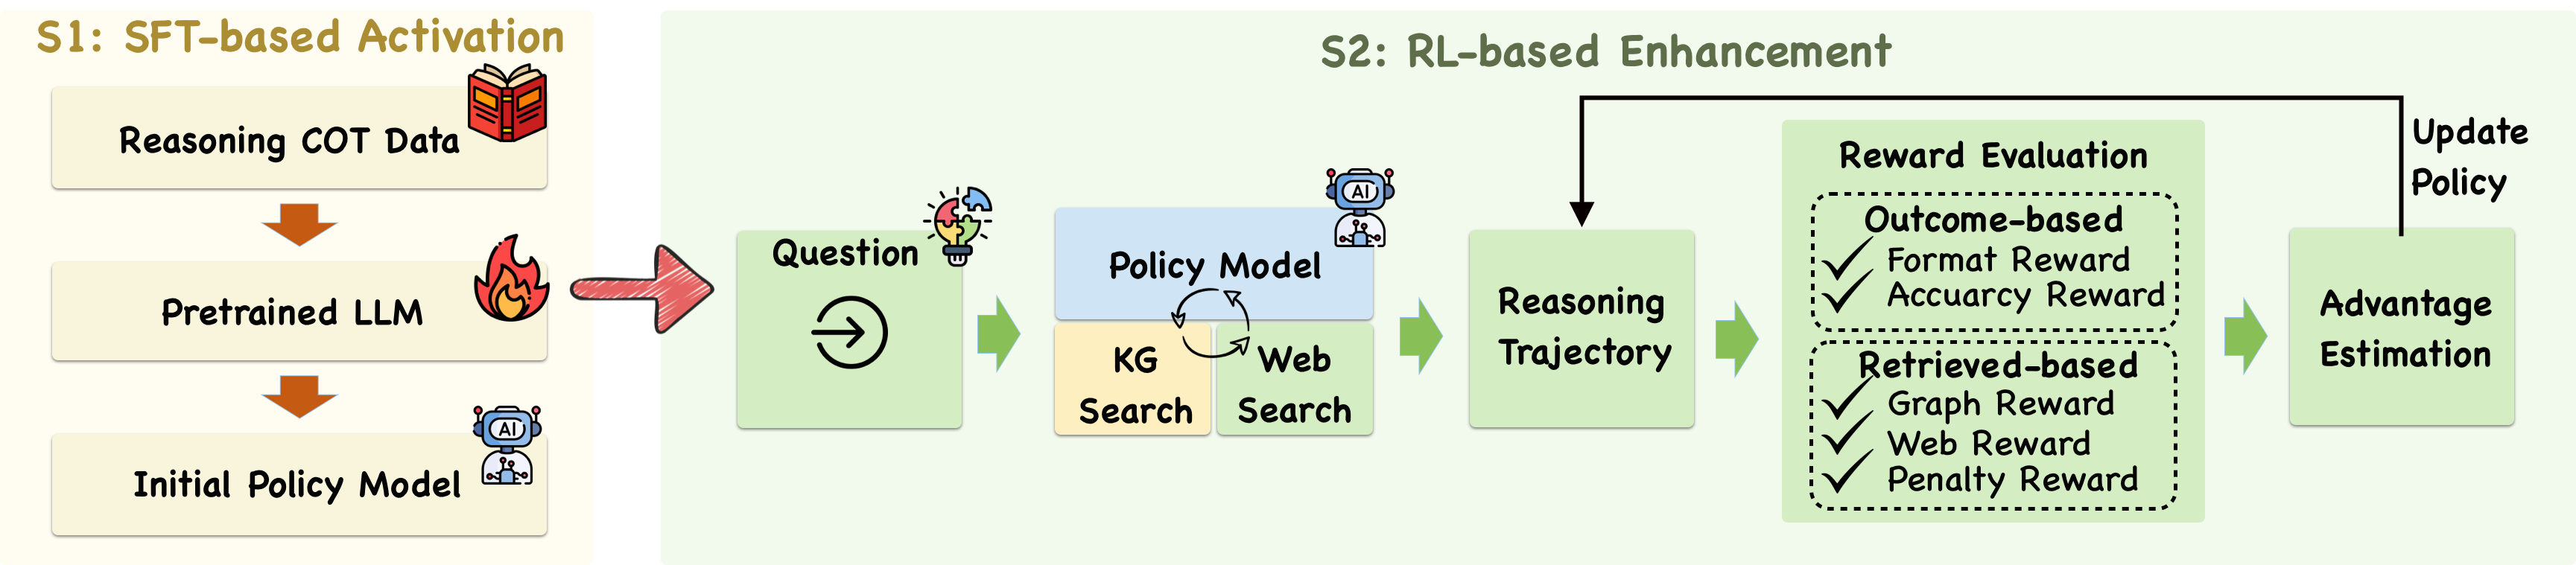
\includegraphics[width=.9\textwidth]{method.png}
    \caption{Graph-RFT Training Framework: SFT-based Reasoning Activation (S1) and RL-based Reasoning Enhancement (S2).}
    \label{frame}
    \vspace{-2ex}
\end{figure*}

\begin{figure*}[t!]
    \centering
    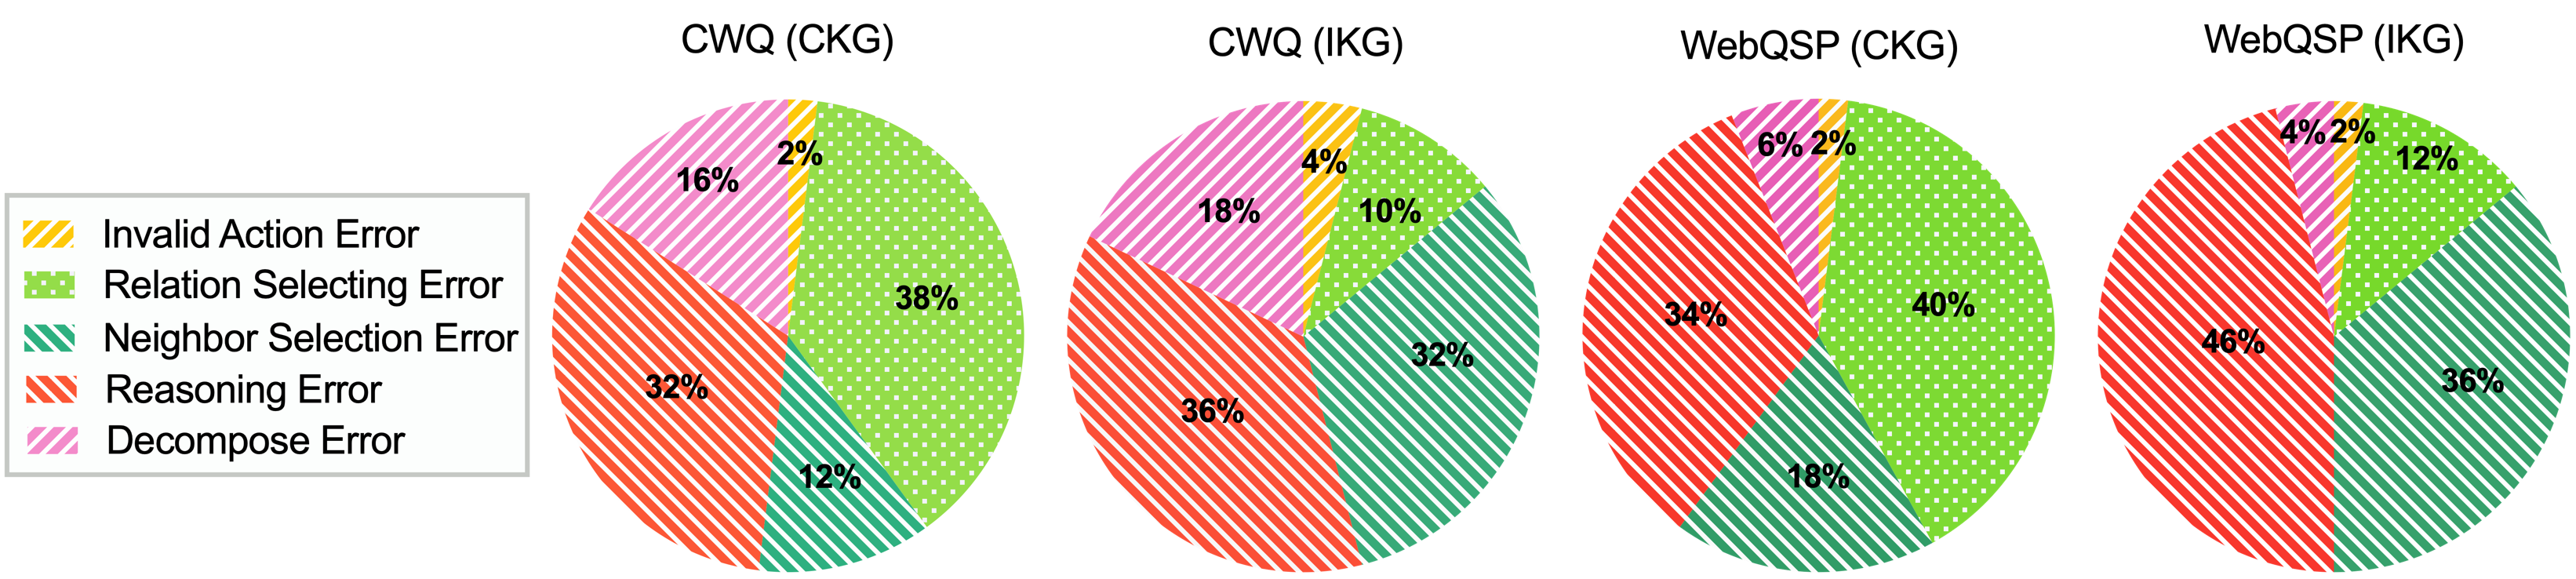
\includegraphics[width=.8\textwidth]{error_type.png}
    \caption{Error Type}
    \label{fig:error}
    \vspace{-2ex}
\end{figure*}

\begin{figure}[H]
    \centering
    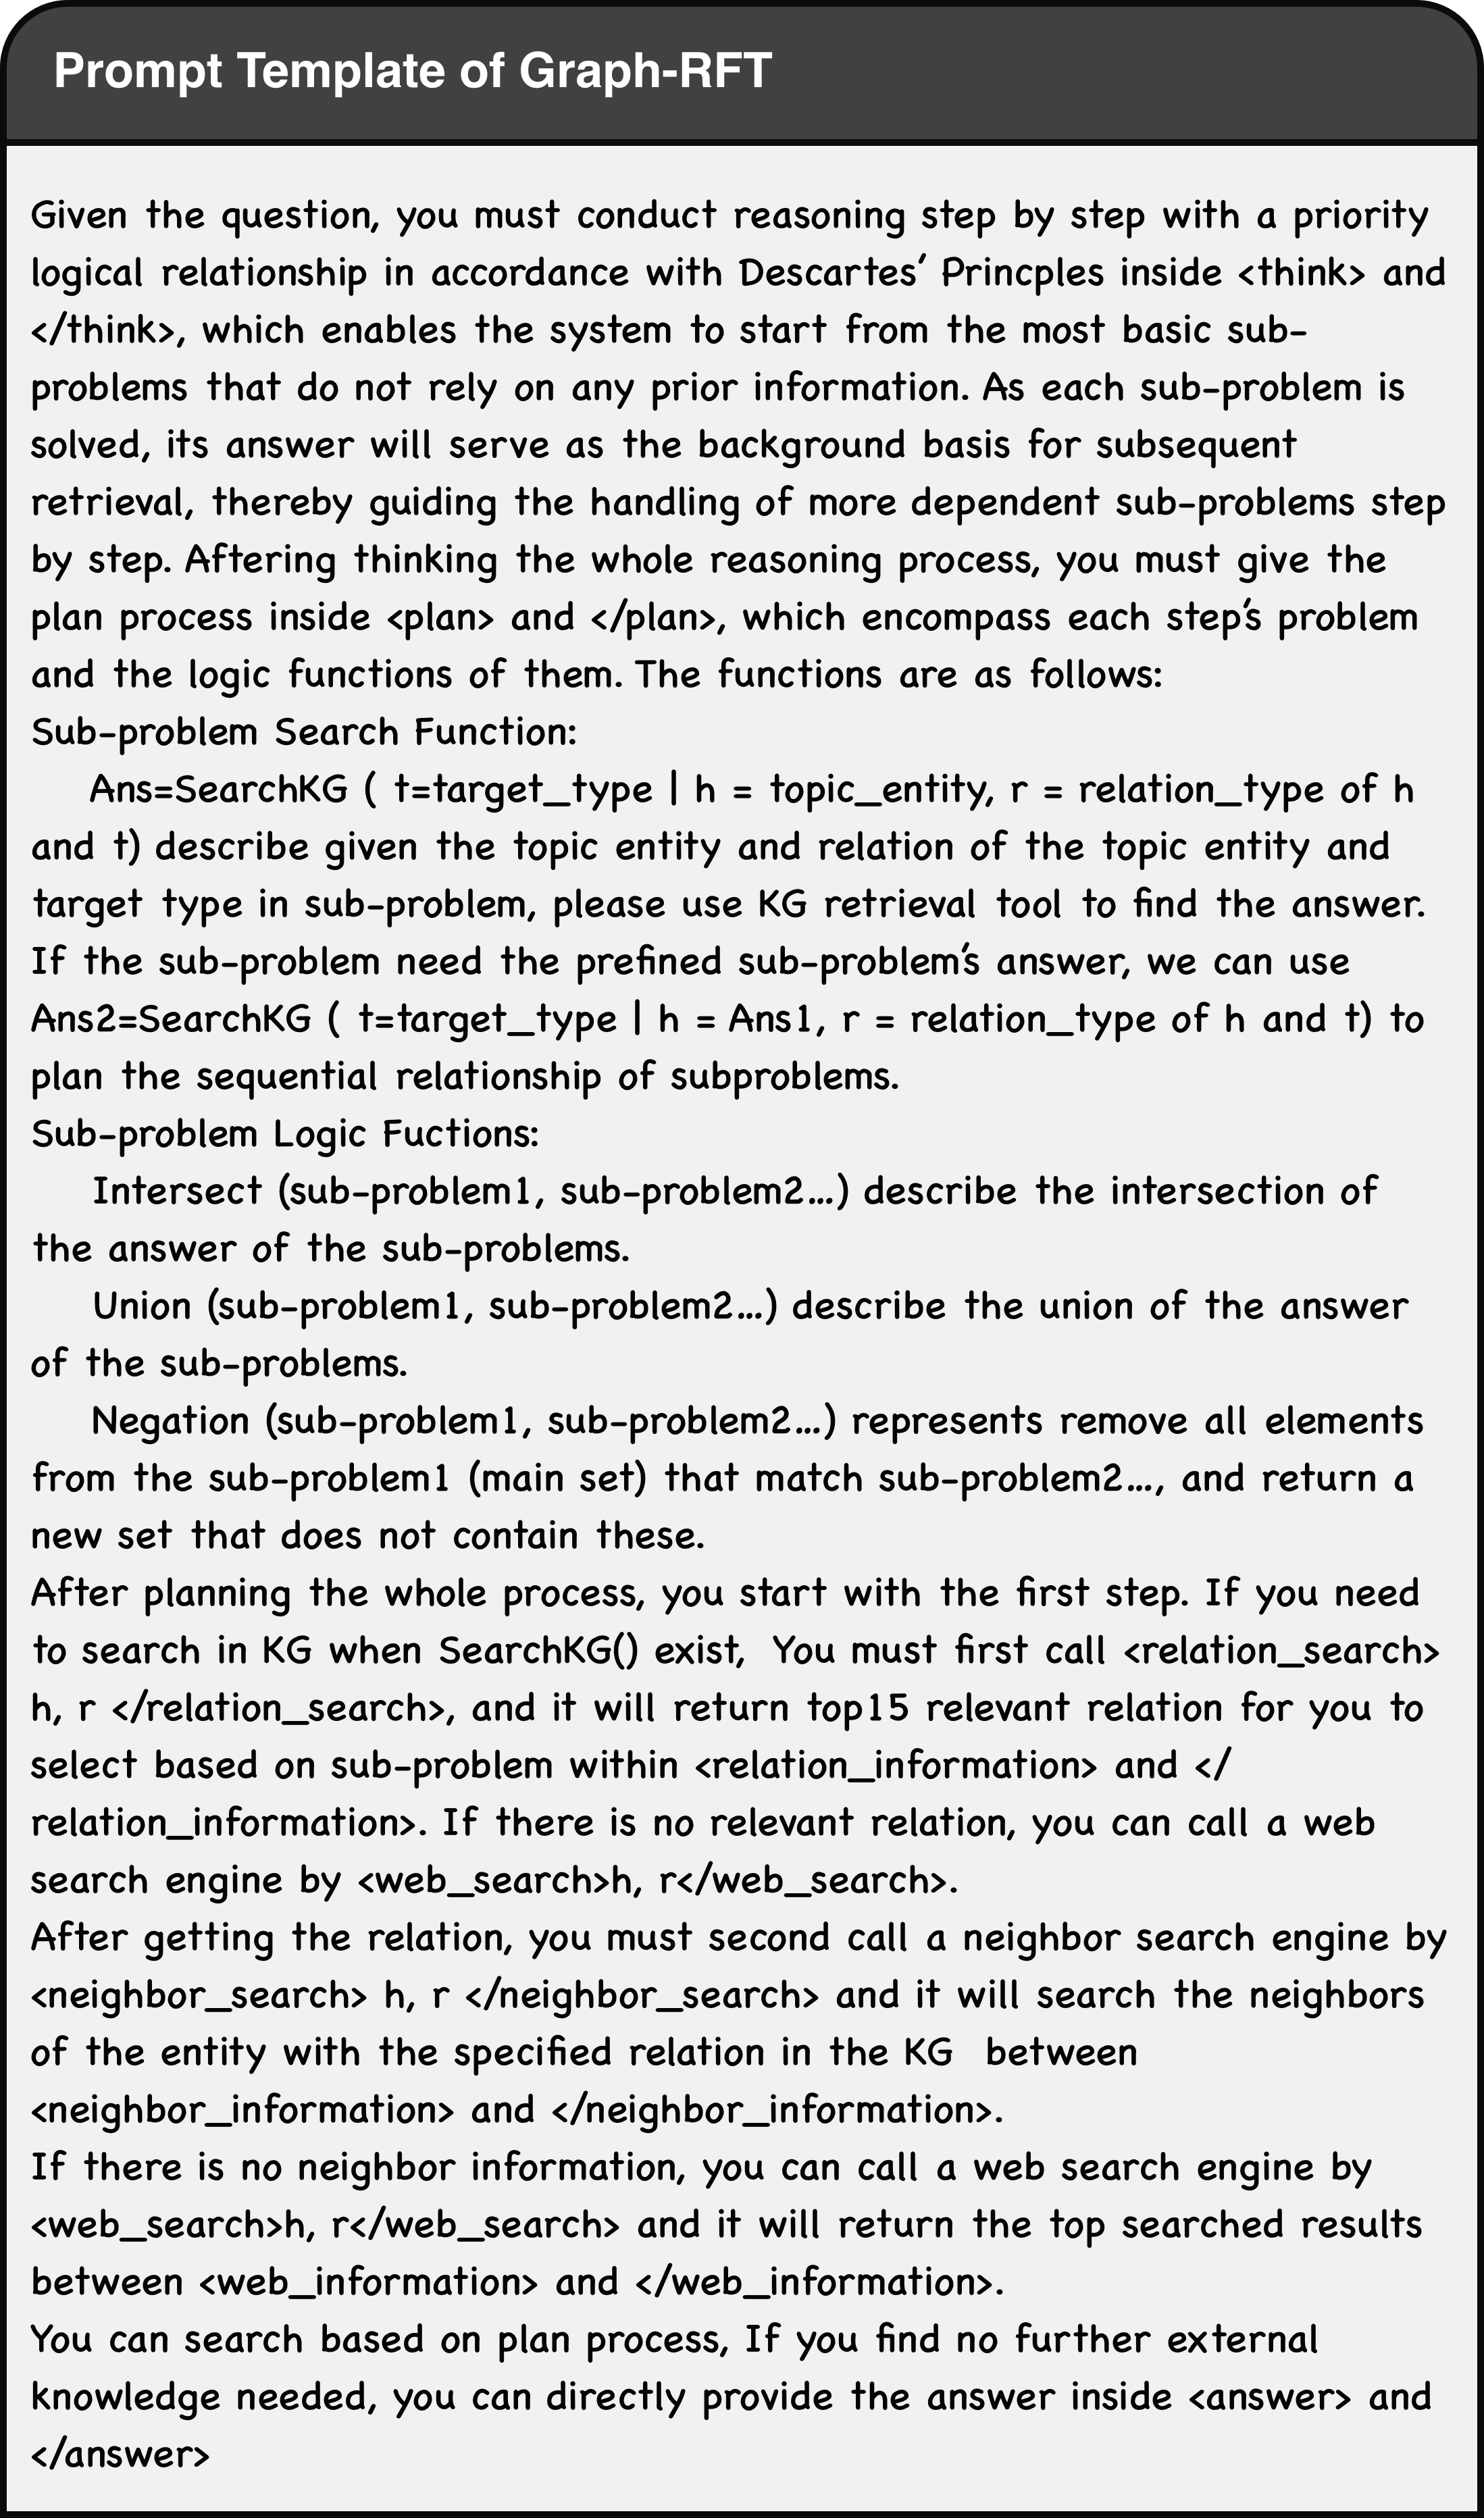
\includegraphics[width=.8\linewidth]{prompt.png}
    \caption{Prompt template of our Graph-RFT.}
    \label{fig:prompt}
\end{figure}

\begin{figure}[H]
    \centering
    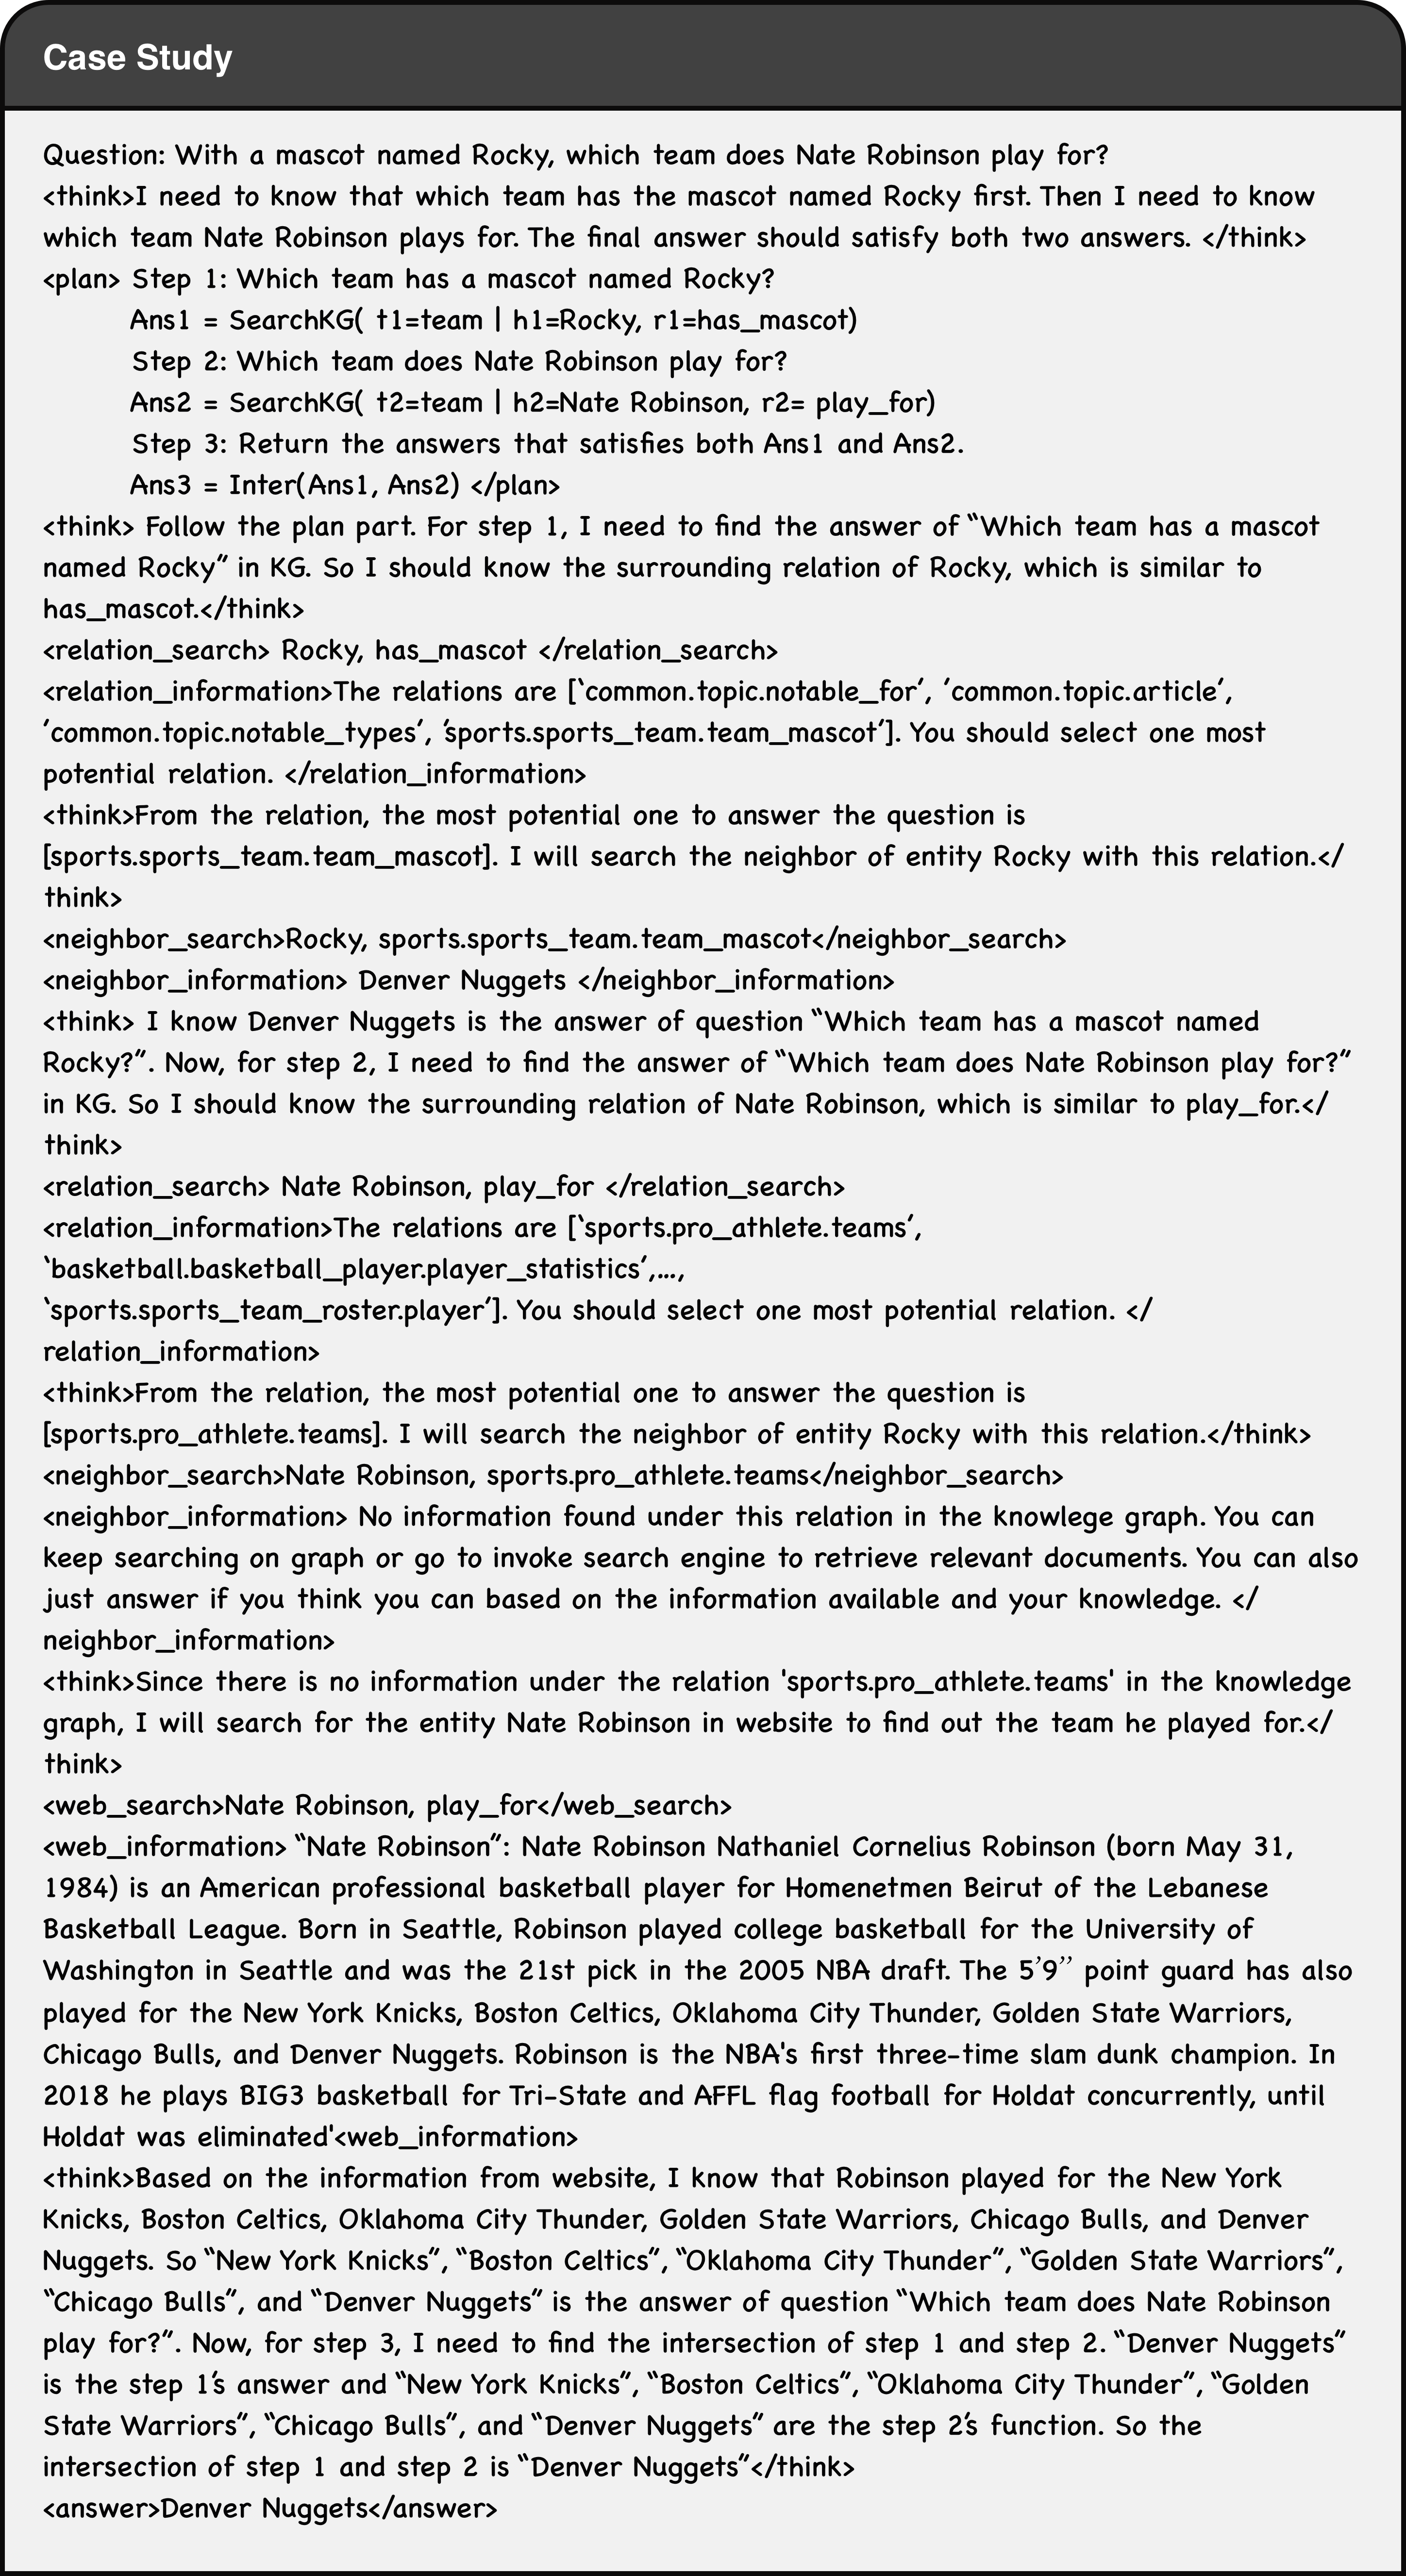
\includegraphics[width=.9\linewidth]{case_study.png}
    \caption{Case Study.}
    \label{fig:case}
\end{figure}

% \subsection{Time Efficiency}
% \label{time}
% To further assess the processing efficiency of Graph-RFT, we carried out extensive evaluations concentrating on the average Hits@1 and running time on the multi-hop question dataset CWQ. Table \ref{app:time} presents a comparison of the performance between ToG and Graph-RFT in the IKG-40\% scenario. The data shows that our model not only has advantages in running efficiency but also achieves better Hits@1 results than ToG, which demonstrates the effectiveness of our model.
% \begin{table}[htbp]
%   \centering
%   \caption{Running time evaluation of ToG and Graph-RFT on CWQ in IKG-40\%.}
%   \label{app:time}
%   \resizebox{\linewidth}{!}{% 可选：自动调整表格宽度以适应页面
%     \begin{tabular}{c|ccccc}
%       \toprule
%       \textbf{Method} &\textbf{Class} & \textbf{Train (min/epoch)} & \textbf{Inference (s/sample)} & \textbf{Hits@1}  \\
%       \midrule
%       ToG & ICL & - & 72.4 & 34.9\\
%       Graph-RFT & RL & 237.4 & 26.3 &67.2\\
%       \bottomrule
%     \end{tabular}
%   }
% \end{table}


% This case allows us to clearly observe the effective collaboration of Graph-RFT’s various components. It also highlights two key capabilities of Graph-RFT: its adaptability to scenarios with incomplete knowledge, and its ability to successfully integrate information from multiple sources to produce accurate answers.


\end{document}
\endinput
%%
%% End of file `sample-sigconf.tex'.
